\documentclass{article}

\usepackage{hyperref}
\usepackage{graphicx} % Required for inserting images
\usepackage[utf8]{inputenc}
\usepackage{listings} % For code listing
\usepackage{xcolor} % For defining colors
\usepackage{subcaption}

\usepackage[left=1.5in, right=1.25in]{geometry}
\usepackage{float}
% Define custom colors for listings
\definecolor{codegreen}{rgb}{0,0.6,0}
\definecolor{codegray}{rgb}{0.5,0.5,0.5}
\definecolor{codepurple}{rgb}{0.58,0,0.82}
\definecolor{backcolour}{rgb}{0.95,0.95,0.92}

% Setup the listings package for code formatting
\lstset{
    backgroundcolor=\color{backcolour},   
    commentstyle=\color{codegreen},
    keywordstyle=\color{magenta},
    numberstyle=\tiny\color{codegray},
    stringstyle=\color{codepurple},
    basicstyle=\ttfamily\footnotesize,
    breakatwhitespace=false,         
    breaklines=true,                 
    captionpos=b,                    
    keepspaces=true,                 
    numbers=left,                    
    numbersep=5pt,                  
    showspaces=false,                
    showstringspaces=false,
    showtabs=false,                  
    tabsize=2
}
\begin{document}
\begin{figure}[htp]
    \centering
    
\includegraphics[width=6cm]{buet_logo.png}
    % \caption{Bangladesh University of Engineering and Technology}
    \label{fig:logo}
\end{figure}

\begin{center}
    \huge{Bangladesh University of Engineering and Technology}
\end{center}

\vspace{1cm}
\begin{center}
    \parbox{\linewidth}{\centering % Horizontally center within the parbox
        \huge \textbf{ZEEK}
    }
\end{center}
\vspace{1cm}
\begin{center}
    \parbox{\linewidth}{\centering % Horizontally center within the parbox
        \Large \textbf{CSE 406 - Computer Security Sessional}
    }
\end{center}

\vspace{1cm}
\begin{flushleft}
\Large \hspace{6pt}\textbf{Team} - \\
\vspace{10pt}
\begin{tabular}{ll} % 'c' for center-aligned, 'l' for left-aligned
\Large \textbf{1905075} & \Large Nahida Marzan 
\\
\Large \textbf{1905086} & \Large Sushmita Paul
% Add more rows as needed
\end{tabular}
\end{flushleft}

\vspace{1cm}
\begin{flushleft}
    \Large \hspace{6pt}\textbf{Supervised by} - Dr. Md. Shohrab Hossain
\end{flushleft}

\tableofcontents
\section{Introduction}
\subsection{Overview}
Zeek is a passive, open-source network traffic analyzer extensively utilized in the realm of network security monitoring (NSM) and a plethora of other traffic analysis tasks. Originally developed for security investigations, Zeek's capabilities transcend to performance measurement and network troubleshooting, offering users a comprehensive view of their network activity through detailed logs and analysis features.
\subsubsection{Comprehensive Logging}
One of the primary advantages of using Zeek is its ability to produce extensive logs that capture a detailed record of network activities. These logs include:
\begin{itemize}
    \item Application-layer transcripts such as HTTP sessions, with details like URIs, headers, MIME types, and server responses.
    \item DNS requests and responses.
    \item SSL certificate information.
    \item Key content from SMTP sessions.
\end{itemize}
Zeek formats these logs in structured, tab-separated, or JSON files, making them ideal for post-processing with external software or integration with databases and SIEM products for further analysis.


\subsubsection{Built-in Analysis and Detection Capabilities}
Zeek is not just about logging; it offers built-in functions for various analysis and detection tasks, such as:
\begin{itemize}
    \item Extracting files from HTTP sessions.
    \item Detecting malware by interfacing with external registries.
    \item Identifying vulnerable software versions and popular web applications on the network.
    \item Detecting SSH brute-force attacks and validating SSL certificate chains.
\end{itemize}
These functionalities are readily available "out of the box," enhancing Zeek's utility as a network analysis tool.

\subsubsection{Customization and Extensibility}
Zeek stands out for its customizability and extensibility, thanks to its domain-specific scripting language. This language allows users to:
\begin{itemize}
    \item Express arbitrary analysis tasks.
    \item Write custom code for unique analysis requirements, extending the pre-built "standard library" that comes with Zeek.
\end{itemize}

This feature positions Zeek as a versatile tool that can adapt to various network monitoring and analysis needs beyond its default offerings.

\subsubsection{High-Performance and Scalability}
Designed to run on commodity hardware, Zeek presents a cost-effective alternative to proprietary network monitoring solutions. Its performance and scalability make it suitable for:
\begin{itemize}
    \item High-speed, high-volume network monitoring, including 10GE and 100GE networks.
    \item Deployment in large-scale environments using Zeek Clusters for load-balancing and centralized management.
\end{itemize}
 Zeek's scalability is one of its core strengths, allowing it to accommodate growing network demands without compromising on performance.
 \subsubsection{Comparison with Other Tools}
 While Zeek excels in generating high-fidelity network logs and analysis, it is distinct from:

 \begin{itemize}
     \item Signature-based IDS systems like Suricata, as Zeek adopts a broader approach to detecting malicious activity through scripting.
     \item Protocol analyzers like Wireshark, which focus on detailed frame-level traffic representation, unlike Zeek's focus on compact, high-fidelity logs.
     \newline
 \end{itemize}
Zeek offers a balanced and efficient solution for network traffic analysis, combining comprehensive logging, built-in analysis capabilities, and extensive customization options. Its adaptability to both small-scale and large-scale environments, along with its open-source nature, makes Zeek a valuable tool for a wide range of users looking to gain deeper insights into their network activity.
\subsection{History of Zeek}

Zeek, initially known as Bro, was developed by Vern Paxson in 1995 at the Lawrence Berkeley National Laboratory (LBNL). Designed as a network monitoring tool, it was coined "Bro" to serve as an Orwellian reminder of the surveillance capabilities inherent in network monitoring, with a nod to the potential for privacy violations.
\\\\
Deployed at LBNL in 1996, Zeek's foundational paper won the Best Paper Award at the USENIX Security Symposium in 1998, reflecting its early recognition and significance in the field of network security.
\\\\
With support from the National Science Foundation (NSF) and the Department of Energy (DOE), the project flourished through a blend of academic research and practical application. As Zeek's user base grew, the need for a more user-friendly interface became apparent, leading to a substantial update with the 2.0 release in 2012, in collaboration with the National Center for Supercomputing Applications (NCSA).
\\\\
Subsequent years saw significant enhancements to Zeek, including native IPv6 support, the creation of the Bro Center of Expertise, the launch of try.zeek.org, and the introduction of the Broker communication framework and Zeek package manager.
\\\\
In 2018, to better reflect its community values and avoid the negative connotations of "bro culture," the project was renamed from Bro to Zeek. Version 3.0, released in 2019, was the first to bear the new name. The year 2020 marked a period of renewed focus on community engagement, with increased outreach efforts aimed at expanding the Zeek community.
\subsection{Optimal Locations for Zeek Deployment}
For effective network monitoring and security analysis, it is crucial to deploy Zeek in strategic locations within the network infrastructure. Below are key points outlining the recommended deployment locations for Zeek:

\begin{enumerate}
    \item \textbf{At Network Perimeters:} Deploy Zeek at the boundaries of the network to monitor all incoming and outgoing traffic, enabling the identification of external threats and unauthorized data exfiltration.
    
    \item \textbf{Core Network Infrastructure:} Position Zeek near central routing and switching devices to capture a broad spectrum of internal network traffic, providing insights into the core network's interactions.
    
    \item \textbf{Data Center Entrances:} Install Zeek at the entry and exit points of data centers to oversee traffic to critical servers and storage systems, safeguarding sensitive information and key assets.
    
    \item \textbf{Network Segmentation Gateways:} Place Zeek at the junctions between different network segments or VLANs to monitor cross-segment traffic, essential for detecting lateral movements and internal threats.
    
    \item \textbf{VPN Concentrators and Access Points:} Deploy Zeek where VPN connections converge or near wireless access points to analyze encrypted and wireless traffic, respectively, ensuring secure remote access and wireless communication.
    
    \item \textbf{Demilitarized Zones (DMZs):} Position Zeek within or adjacent to DMZs to scrutinize traffic between the internet and internal network, protecting services exposed to the outside world.
    
    \item \textbf{Branch Offices:} Extend Zeek deployment to branch or remote offices to monitor localized traffic, ensuring comprehensive network security coverage across all organizational units.
    
    \item \textbf{High Availability Clusters:} In critical network environments, deploy Zeek in a high availability configuration with load balancing to ensure continuous monitoring and redundancy, preventing single points of failure.
\end{enumerate}

% \usepackage{graphicx}
% \usepackage{listings}
% \usepackage{xcolor}
% \usepackage{float}  % Add this line to use [H] option for figure placement

\lstdefinestyle{bashstyle}{
  language=bash,
  basicstyle=\small\ttfamily,
  commentstyle=\color{green!40!black},
  keywordstyle=\color{blue},
  % frame=single,
  breaklines=true,
  postbreak=\mbox{\textcolor{red}{$\hookrightarrow$}\space},
}

\section{Installation}

\begin{enumerate}
 \item \textbf{Install ethtool}
    \begin{lstlisting}[style=bashstyle]
      sudo apt install ethtool
    \end{lstlisting}
  \begin{figure}[H]
  \centering
  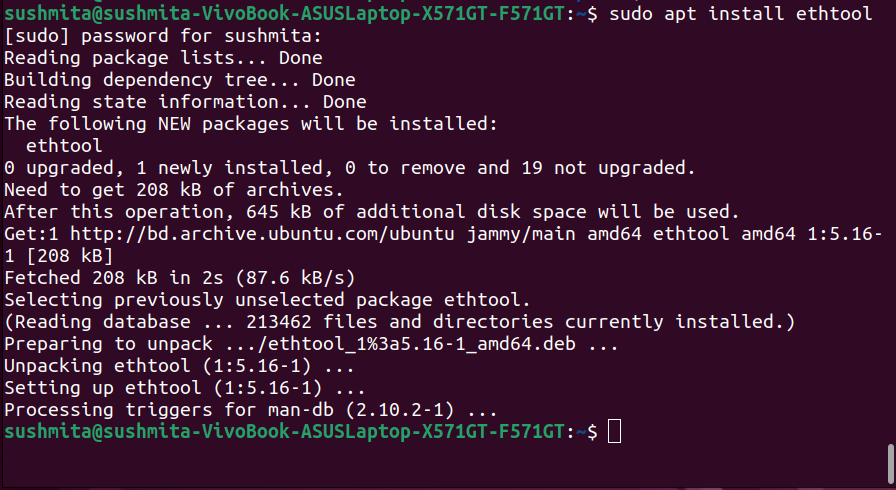
\includegraphics[width=0.8\textwidth]
  {images/install/1_install_ethtool.png}
  \caption{install ethtool}
  \end{figure}
  \item \textbf{Update your system}
    \begin{lstlisting}[style=bashstyle]
      sudo apt-get update
    \end{lstlisting}
    \begin{figure}[H]
    \centering
    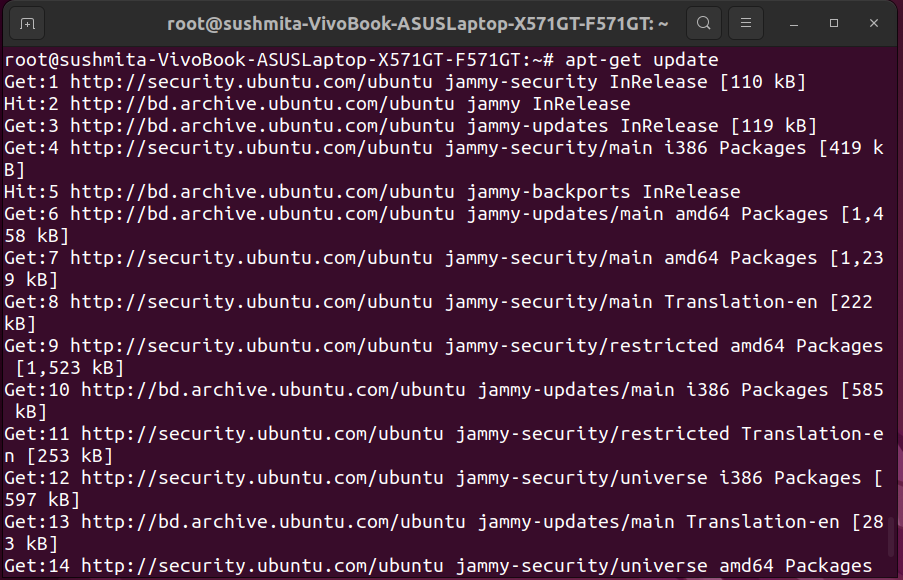
\includegraphics[width=0.8\textwidth]{images/install/2_apt_get_update.png}
    \caption{system update}
\end{figure}
  \item \textbf{Upgrade your system}
    \begin{lstlisting}[style=bashstyle]
      sudo apt-get upgrade
    \end{lstlisting}
    \begin{figure}[H]
  \centering
  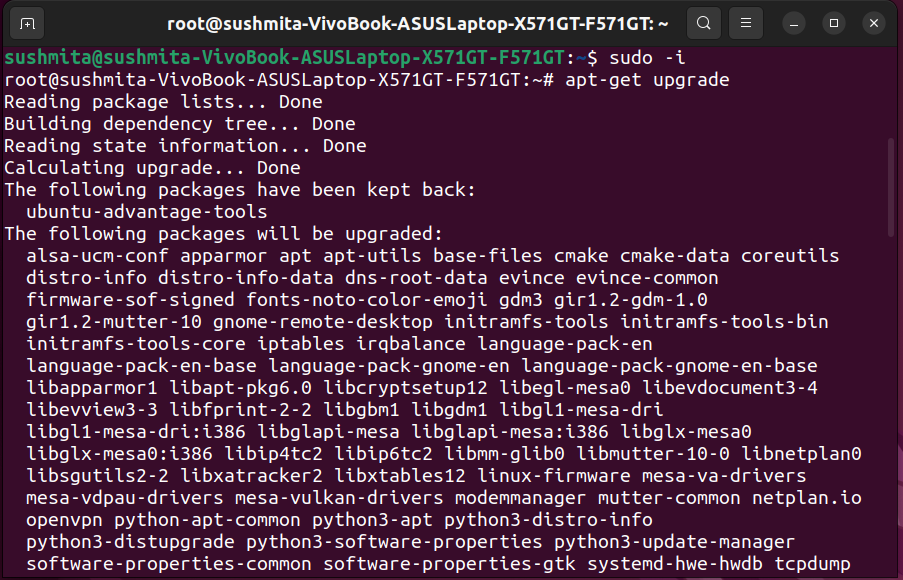
\includegraphics[width=0.8\textwidth]{images/install/3_apt_get_upgrade.png}
  \caption{system upgrade}
\end{figure}
  \item \textbf{Install Zeek pre-req}
    \begin{lstlisting}[style=bashstyle]
      sudo apt-get install cmake make gcc g++ flex bison libpcap-dev libssl-dev python2-dev swig zlib1g-dev
    \end{lstlisting}
    \begin{figure}[H]
  \centering
  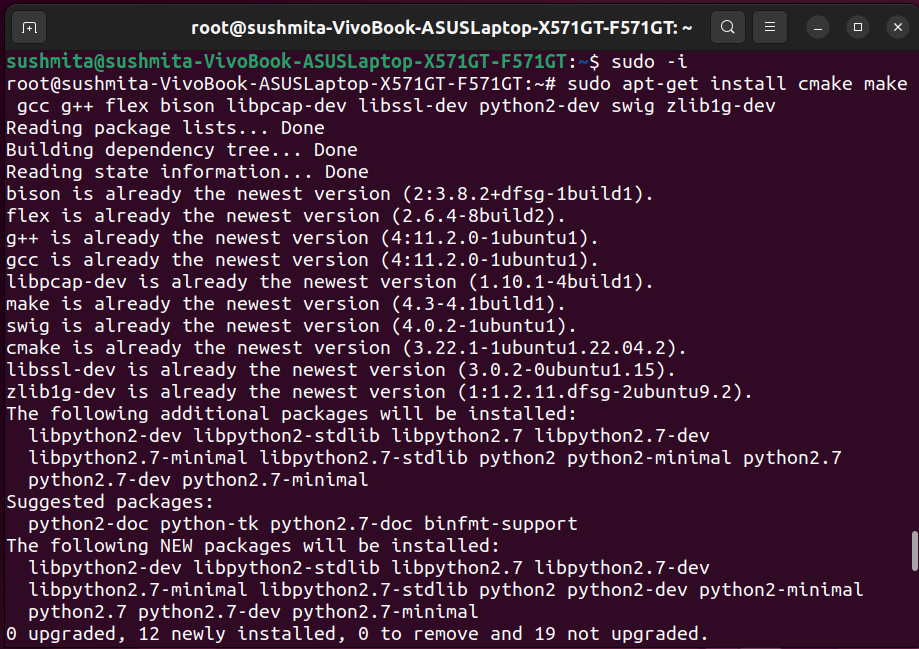
\includegraphics[width=0.8\textwidth]{images/install/4_zeek_prereq_install.png}
  \caption{Zeek pre-req}
\end{figure}
\item \textbf{Check ubuntu version}
    \begin{lstlisting}[style=bashstyle]
      lsb_release -a
    \end{lstlisting}
    \begin{figure}[H]
  \centering
  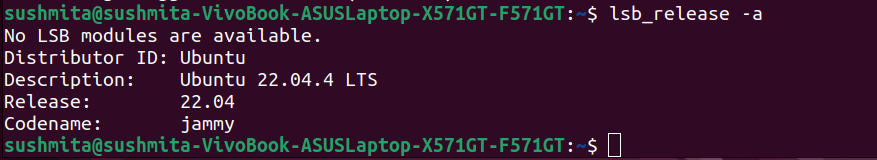
\includegraphics[width=0.8\textwidth]{images/install/5_check_ubuntu_version.png}
  \caption{ubuntu version}
  \end{figure}
  \item \textbf{Add Zeek repositories to local repositories}
    \begin{lstlisting}[style=bashstyle]
      wget -nv https://download.opensuse.org/repositories/security:/zeek/xUbuntu_22.04/Release.key -O Release.key
    \end{lstlisting}
    \begin{figure}[H]
  \centering
  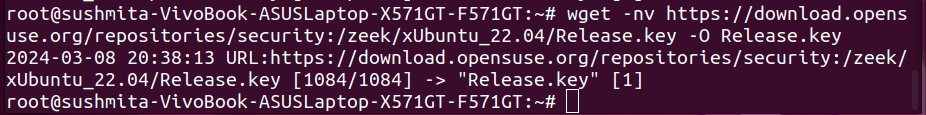
\includegraphics[width=0.8\textwidth]{images/install/6_add_zeek_repo_to_local_repo.png}
  \caption{add zeek repo}
\end{figure}
  \item \textbf{Add key}
    \begin{lstlisting}[style=bashstyle]
      sudo apt-key add -< Release.key
    \end{lstlisting}
    \begin{figure}[H]
  \centering
  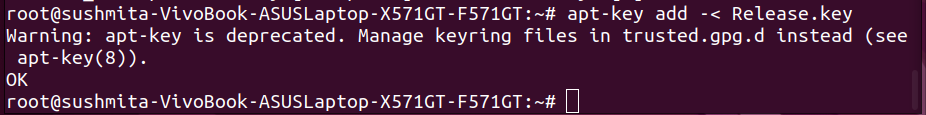
\includegraphics[width=0.8\textwidth]{images/install/7_add_key.png}
  \caption{add key}
\end{figure}
  \item \textbf{Update package to see if there's a new repo}
    \begin{lstlisting}[style=bashstyle]
      sudo apt-get update
    \end{lstlisting}
    \begin{figure}[H]
  \centering
  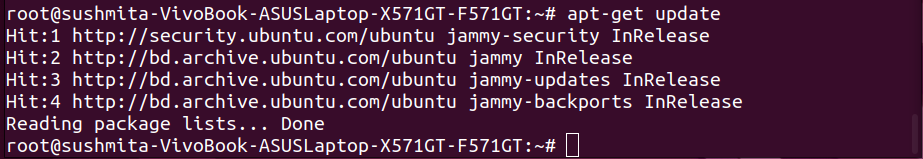
\includegraphics[width=0.8\textwidth]{images/install/8_update_after_addkey.png}
  \caption{update after add key}
\end{figure}
  \item \textbf{Add repo}
    \begin{lstlisting}[style=bashstyle]
      sudo sh -c "echo 'deb http://download.opensuse.org/repositories/security:/zeek/xUbuntu_22.04/ /' > /etc/apt/sources.list.d/security:zeek.list"
    \end{lstlisting}
    \begin{figure}[H]
  \centering
  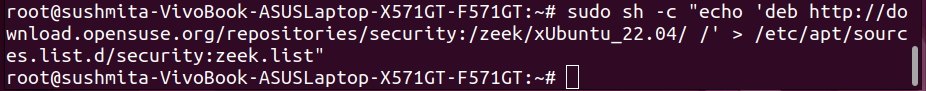
\includegraphics[width=0.8\textwidth]{images/install/9_add_repo.png}
  \caption{add repo}
\end{figure}
  \item \textbf{Update to see if we have any new repo}
    \begin{lstlisting}[style=bashstyle]
      sudo apt-get update
    \end{lstlisting}
    \begin{figure}[H]
  \centering
  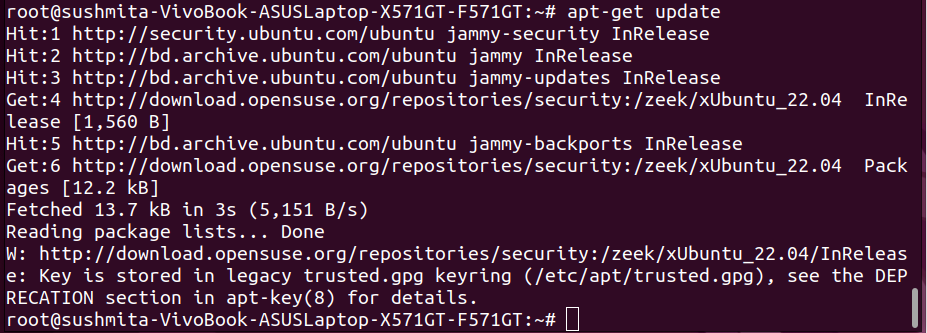
\includegraphics[width=0.8\textwidth]{images/install/10_update_to_see_new_repo.png}
  \caption{update}
\end{figure}
  \item \textbf{Install Zeek}
    \begin{lstlisting}[style=bashstyle]
      sudo apt-get install zeek-lts
    \end{lstlisting}
  \item \textbf{Zeek is now installed!}
  \begin{figure}[H]
  \centering
  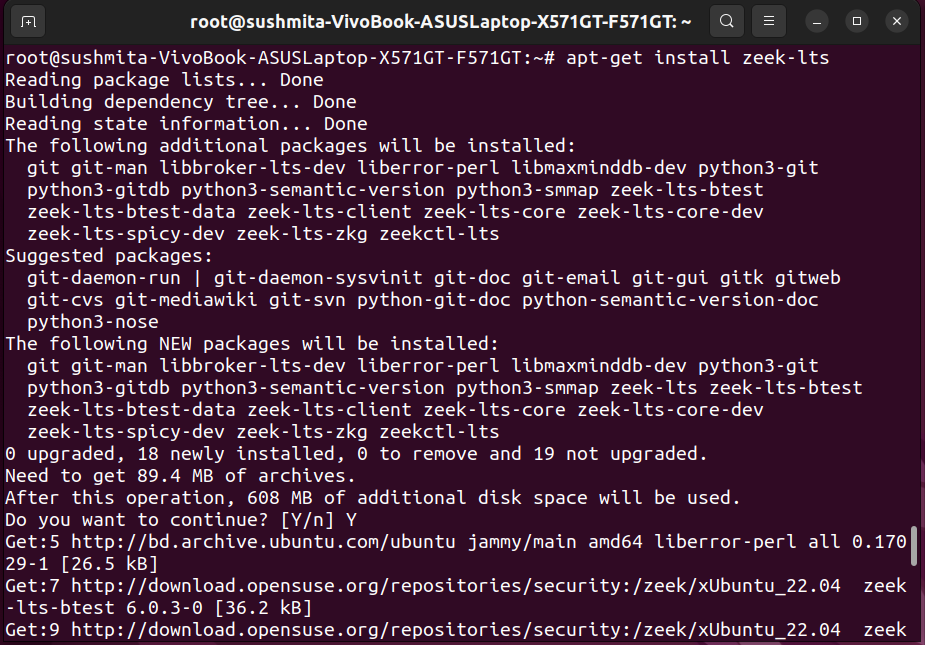
\includegraphics[width=0.8\textwidth]{images/install/11_install_zeek.png}
  \caption{install zeek}
\end{figure}
  \item \textbf{To verify if we have installed}
    \begin{lstlisting}[style=bashstyle]
      ls /opt/
      cd /opt/zeek
      ls
      cd bin/
      ./zeek -h
      ./zeekctl -h
    \end{lstlisting}
  \item \textbf{Installation is verified!}
  \begin{figure}[H]
  \centering
  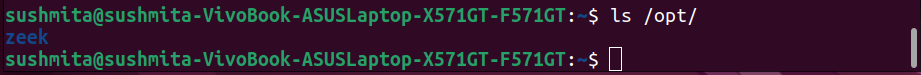
\includegraphics[width=0.8\textwidth]{images/install/12_install_verification.png}
  \caption{Zeek Installation Verification 1}
  \end{figure}
  \begin{figure}[H]
  \centering
  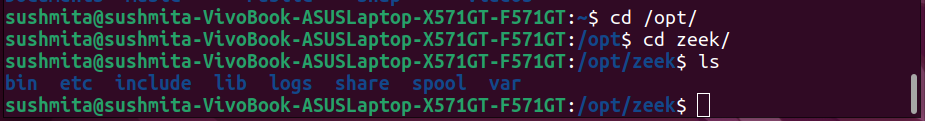
\includegraphics[width=0.8\textwidth]{images/install/13_install_verification.png}
  \caption{Zeek Installation Verification 2}
  \end{figure}
  \begin{figure}[H]
  \centering
  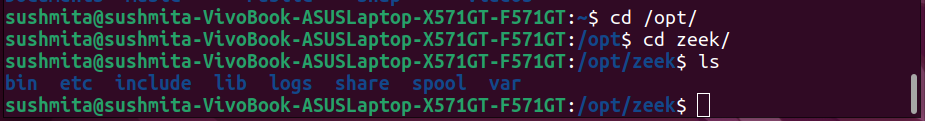
\includegraphics[width=0.8\textwidth]{images/install/13_install_verification.png}
  \caption{Zeek Installation Verification 3}
  \end{figure}
\end{enumerate}

\section{Architecture of Zeek}
Zeek, formerly known as Bro, is a powerful network analysis tool that is distinguished by its unique architecture. This architecture is primarily divided into two major components: the event engine, which processes incoming network traffic, and the script interpreter, which applies user-defined scripts to the processed data. This high-level overview aims to elucidate the roles and functionalities of these components within Zeek's architecture.

\begin{figure}[h]
    \centering
    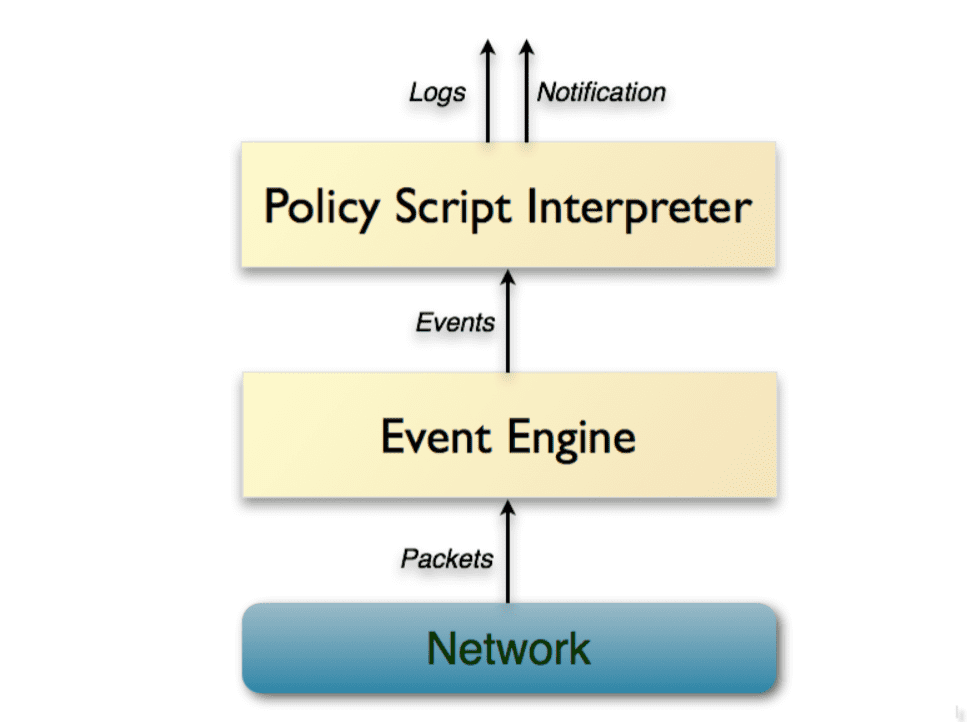
\includegraphics[width=0.5\linewidth]{images/architecture.PNG}
    \caption{Architecture of Zeek}
    \label{fig:enter-label}
\end{figure}

\subsection{Event Engine}

The event engine, or core, of Zeek plays a pivotal role in transforming the raw stream of network packets into structured, high-level events. These events are designed to be policy-neutral, focusing solely on the activities observed within the network without imparting any judgment or significance.

\subsubsection{Subcomponents of the Event Engine}

The event engine is further divided into several key subcomponents, each responsible for a specific aspect of packet processing:

\begin{itemize}
    \item \textbf{Input Sources:} This subcomponent is tasked with ingesting incoming network traffic from various network interfaces.
    \item \textbf{Packet Analysis:} Starting at the link layer, this process involves the analysis of lower-level protocols to dissect the network traffic.
    \item \textbf{Session Analysis:} Focused on application-layer protocols (e.g., HTTP, FTP), session analysis examines the content and context of communication sessions.
    \item \textbf{File Analysis:} This involves the inspection of file content being transferred over the network, providing insights into the data being exchanged.
\end{itemize}

The modularity and plugin architecture of the event engine enable the integration and expansion of Zeek's capabilities, allowing for customized enhancements beyond the core code base.

\subsection{Script Interpreter}

Complementing the event engine is the script interpreter, a critical component that leverages Zeek's custom scripting language to process the events generated by the event engine. This interpreter facilitates the implementation of a site's security policies and the derivation of network statistics.

\subsubsection{Functionality of the Script Interpreter}

The script interpreter offers a wide range of capabilities, including but not limited to:

\begin{itemize}
    \item \textbf{Security Policy Enforcement:} Through the execution of event handlers, scripts can define and enforce security measures in response to detected network activities.
    \item \textbf{Statistical Analysis:} Scripts are capable of extracting and analyzing various properties and statistics from the network traffic, enriching the understanding of network behavior.
    \item \textbf{State Management:} Zeek's scripting language allows for the maintenance of state over time, enabling the tracking and correlation of network events across different connections and hosts.
    \item \textbf{Alert Generation:} The script interpreter can produce real-time alerts and trigger external programs, facilitating proactive responses to potential security threats.
\end{itemize}



Zeek's architecture, characterized by its event engine and script interpreter, provides a robust foundation for the processing and analysis of network traffic. This design enables Zeek to deliver comprehensive insights into network activities, supporting a broad spectrum of security and monitoring applications.

\section{Functionality of Zeek}
Zeek stands out as a versatile platform for network security and analysis for several compelling reasons:
\begin{enumerate}
    \item \textbf{Focused on Network Data:} Specialization in collecting and analyzing network data, a critical component for security teams.
    
    \item \textbf{Diverse Data Collection:} Support for various data types including transaction data, extracted content, and alert data, as defined by the network security monitoring paradigm.
    
    \item \textbf{Rich Transaction Logs:} Default generation of detailed, high-fidelity, and richly-annotated transaction logs, offering a neutral view of network activities.
    
    \item \textbf{File Extraction Capabilities:} Robust features for carving files from network traffic, facilitating further analysis with various tools.
    
    \item \textbf{Alert Mechanism:} Provision of an alert system through the notice mechanism, enabling judgment on network traffic.
    
    \item \textbf{Customization and Extensibility:} Availability of a domain-specific scripting language for tailoring functionalities to specific analysis needs.
    
    \item \textbf{Cost-Effective Deployment:} Ability to run on commodity hardware, making it an accessible solution for organizations of all sizes.
    
    \item \textbf{Comprehensive Analysis and Detection:} Inclusion of built-in functionalities for a wide array of analysis and detection tasks, enhancing its utility as an analysis tool.
\end{enumerate}

\section{Log files in Zeek}
\subsection{conn.log}
The conn.log in Zeek is crucial for tracking network connections, covering both stateful protocols like TCP and stateless ones like UDP. It provides a comprehensive view of network interactions, detailing each connection's aspects. Analysts use this log to understand network behavior, identify anomalies, and investigate incidents. 
\begin{lstlisting}[language=Python, caption= conn.log entry]
{
  "ts": 1591367999.430166,
  "uid": "C5bLoe2Mvxqhawzqqd",
  "id.orig_h": "192.168.4.76",
  "id.orig_p": 46378,
  "id.resp_h": "31.3.245.133",
  "id.resp_p": 80,
  "proto": "tcp",
  "service": "http",
  "duration": 0.25411510467529297,
  "orig_bytes": 77,
  "resp_bytes": 295,
  "conn_state": "SF",
  "missed_bytes": 0,
  "history": "ShADadFf",
  "orig_pkts": 6,
  "orig_ip_bytes": 397,
  "resp_pkts": 4,
  "resp_ip_bytes": 511
}
\end{lstlisting}
A conversation between 192.168.4.76 and 31.3.245.133 occurred on Jun 5, 2020, at 14:39:59 UTC, lasting only 0.254 seconds. They communicated via HTTP on TCP port 80, with 192.168.4.76 sending 77 bytes at the application layer and 397 bytes at the IP layer.

\subsection{dns.log}
Zeek's dns.log captures DNS queries and responses, recording details such as the querying host, the DNS server, the requested domain, and the response. It's used for security and network analysis, helping to identify normal and malicious DNS activities, including domain resolutions and potential misuse of DNS for command-and-control or data exfiltration purposes.
\begin{lstlisting}[language=Python, caption= dns.log entry]
{
  "ts": 1591367999.305988,
  "uid": "CMdzit1AMNsmfAIiQc",
  "id.orig_h": "192.168.4.76",
  "id.orig_p": 36844,
  "id.resp_h": "192.168.4.1",
  "id.resp_p": 53,
  "proto": "udp",
  "trans_id": 19671,
  "rtt": 0.06685185432434082,
  "query": "testmyids.com",
  "qclass": 1,
  "qclass_name": "C_INTERNET",
  "qtype": 1,
  "qtype_name": "A",
  "rcode": 0,
  "rcode_name": "NOERROR",
  "AA": false,
  "TC": false,
  "RD": true,
  "RA": true,
  "Z": 0,
  "answers": [
    "31.3.245.133"
  ],
  "TTLs": [
    3600
  ],
  "rejected": false
}
\end{lstlisting}
According to this log entry, 192.168.4.76 asked 192.168.4.1 for the A record of the host testmyids.com, and received the answer 31.3.245.133. 

\subsection{http.log}
Zeek's http.log captures details of HTTP and exposed HTTPS traffic, recording request and response information like methods, URIs, status codes, and MIME types. It's valuable for analyzing web activities, identifying suspicious or malicious behavior, and correlating with other logs like conn.log for comprehensive network insight.
\begin{lstlisting}[language=Python, caption= http.log entry]
{
  "ts": 1591367999.512593,
  "uid": "C5bLoe2Mvxqhawzqqd",
  "id.orig_h": "192.168.4.76",
  "id.orig_p": 46378,
  "id.resp_h": "31.3.245.133",
  "id.resp_p": 80,
  "trans_depth": 1,
  "method": "GET",
  "host": "testmyids.com",
  "uri": "/",
  "version": "1.1",
  "user_agent": "curl/7.47.0",
  "request_body_len": 0,
  "response_body_len": 39,
  "status_code": 200,
  "status_msg": "OK",
  "tags": [],
  "resp_fuids": [
    "FEEsZS1w0Z0VJIb5x4"
  ],
  "resp_mime_types": [
    "text/plain"
  ]
}
\end{lstlisting}
A request from 192.168.4.76 to 31.3.245.133 was logged by Zeek, showing a HTTP GET request to testmyids.com. The response was "200 OK" with MIME type "text/plain." Zeek assigned a file ID to this exchange, allowing content review if configured. The unique connection ID links this HTTP interaction to the corresponding conn.log entry, facilitating comprehensive network analysis.

\subsection{files.log}
Zeek's files.log records observed files in network traffic, detailing their types and transactions. Analysts can configure Zeek to extract and save specific file types, like executables, for further analysis. This process is tracked through conn.log and http.log to understand file transfer contexts.
\begin{lstlisting}[language=Python, caption= files.log entry]
{
  "ts": 1596820191.969902,
  "fuid": "FBbQxG1GXLXgmWhbk9",
  "uid": "CzoFRWTQ6YIzfFXHk",
  "id.orig_h": "192.168.4.37",
  "id.orig_p": 58264,
  "id.resp_h": "23.195.64.241",
  "id.resp_p": 80,
  "source": "HTTP",
  "depth": 0,
  "analyzers": [
    "EXTRACT",
    "PE"
  ],
  "mime_type": "application/x-dosexec",
  "duration": 0.015498876571655273,
  "is_orig": false,
  "seen_bytes": 179272,
  "total_bytes": 179272,
  "missing_bytes": 0,
  "overflow_bytes": 0,
  "timedout": false,
  "extracted": "HTTP-FBbQxG1GXLXgmWhbk9.exe",
  "extracted_cutoff": false
}
\end{lstlisting}
The files.log entry in Zeek includes a UID from conn.log, linking the file activity to a specific connection. Zeek activated file extraction and analysis, successfully handling 179272 bytes without loss, and saved the file as HTTP-FBbQxG1GXLXgmWhbk9.exe. The is orig field indicates the file's sender; here, the HTTP server at 23.195.64.241 sent the file to 192.168.4.37.
\subsection{ftp.log}
Zeek's ftp.log records FTP communications, detailing client-server interactions including login credentials, commands, and file transfers. It captures both control channel activities and file transfer specifics, highlighting FTP's use of separate TCP connections for commands and data.

\subsection{ssl.log}
Zeek's ssl.log captures metadata for TLS-encrypted sessions, including TLS versions, cipher suites, and elliptic curves. It's critical for understanding the security posture of encrypted communications, offering insights into protocol usage and potential vulnerabilities without decrypting traffic.
\begin{lstlisting}[language=Python, caption= ssl.log entry]
{
  "ts": 1598377391.921726,
  "uid": "CsukF91Bx9mrqdEaH9",
  "id.orig_h": "192.168.4.49",
  "id.orig_p": 56718,
  "id.resp_h": "13.32.202.10",
  "id.resp_p": 443,
  "version": "TLSv12",
  "cipher": "TLS_ECDHE_RSA_WITH_AES_128_GCM_SHA256",
  "curve": "secp256r1",
  "server_name": "www.taosecurity.com",
  "resumed": false,
  "next_protocol": "h2",
  "established": true,
  "cert_chain_fuids": [
    "F2XEvj1CahhdhtfvT4",
    "FZ7ygD3ERPfEVVohG9",
    "F7vklpOKI4yX9wmvh",
    "FAnbnR32nIIr2j9XV"
  ],
  "client_cert_chain_fuids": [],
  "subject": "CN=www.taosecurity.com",
  "issuer": "CN=Amazon,OU=Server CA 1B,O=Amazon,C=US"
}
\end{lstlisting}
This log entry captures a TLS 1.2 handshake between a client and a server, specifying the use of the ECDHE\_RSA key exchange with AES\_128\_GCM\_SHA256 encryption and the secp256r1 elliptic curve. It indicates a connection to "www.taosecurity.com", authenticated with a certificate chain issued by Amazon. The connection upgrades to HTTP/2 ("h2"). No client certificates are used in this session. The log is part of a series, with certificate details to be analyzed in an upcoming x509 log entry.

\subsection{x509.log}
Zeek's x509.log records details from TLS certificates exchanged during secure connections, providing insights into the security of these connections, including the certificate chain and key details. This log is particularly valuable for analyzing certificate validity, issuer authenticity, and encryption standards used in network communications.

\subsection{smtp.log}
Zeek logs SMTP traffic, providing insights into email transactions over various ports, including encrypted ones. It identifies key elements like sender, receiver, and authentication details, even in encrypted sessions, aiding in network security analysis.

\subsection{ssh.log}
Zeek's SSH log provides insights into SSH sessions, detailing aspects like authentication success, encryption types, and client-server interactions, aiding in the analysis of secure remote connections and potential lateral movements within networks.
\subsection{pe.log}
pe.log entry provides details about a portable executable file, including its architecture, operating system compatibility, security features, and structural components. It helps analysts understand the essential characteristics of the executable file quickly.


\subsection{dhcp.log}
dhcp.log provides detailed information about a DHCP (Dynamic Host Configuration Protocol) exchange between a client and a server. It captures the Discover-Offer-Request-Acknowledge (DORA) process, showing the messages exchanged between the client and server, including requests for IP addresses, server responses, assigned IP addresses, lease durations, and other configuration parameters. Additionally, it explains how tools like tcpdump, tshark, and Zeek (formerly known as Bro) can be used to analyze and interpret DHCP exchanges for network and security purposes.

\subsection{weird.log}
weird.log is various random stuff where analyzers ran into trouble understanding the traffic in terms of their protocols; basically whenever there’s something unexpected at the protocol level, that’s a weird (for a lack of anything better to do with it). That means that “weirds” are also essentially hardcoded by whoever wrote that analyzer. They can also be generated by scripts, but that’s rarer.

\subsection{notice.log}
notice.log on the other hand are situations explicitly detected and reported by Zeek scripts as inspection-worthy. It’s usually not protocol errors, but something semantically higher (like a self-signed cert). Notices are part of the script-level analysis and can be raised by Zeek packages as well.





\section{Network Monitoring :}
\subsection{Live Network Monitoring:}
\subsubsection{Simulation :}


\begin{itemize}
    \item Determine the active network interfaces on the system by executing the ip a command. This step is essential for identifying the interface through which network traffic will be monitored.
\end{itemize}

\begin{figure}[H]
    \centering
    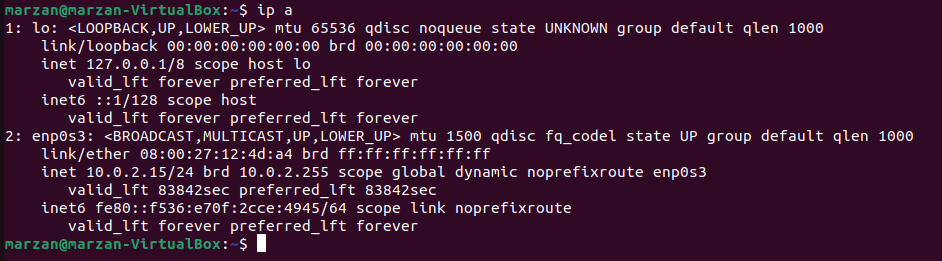
\includegraphics[width=1\linewidth]{images/ipa.png}
    \caption{live network interfaces}
    \label{fig:enter-label}
\end{figure}

\begin{itemize}
    \item Configure the Zeek node by editing the node.cfg file. Specify the network interface to be monitored by adding the line interface=enp0s3.
\end{itemize}


\begin{figure}[H]
    \centering
    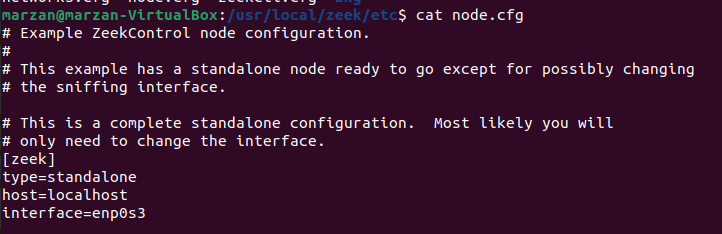
\includegraphics[width=1\linewidth]{images//live_monitor/node.png}
    \caption{node.cfg update}
    \label{fig:enter-label}
\end{figure}

\begin{itemize}
    \item Utilize the zeekctl command-line utility to manage the Zeek instance. Initiate Zeek by executing zeekctl start, and when necessary, halt the monitoring process using zeekctl stop.
\end{itemize}


\begin{figure}[H]
    \centering
    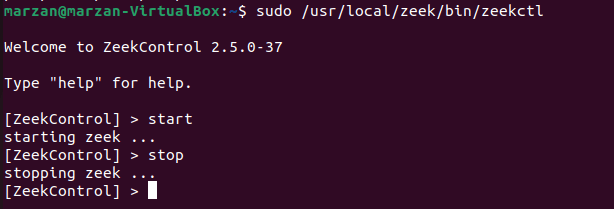
\includegraphics[width=1\linewidth]{images/live_monitor/zeekctl.png}
    \caption{zeekctl}
    \label{fig:enter-label}
\end{figure}

\begin{itemize}
    \item To ascertain the installation path of the zeekctl utility, employ the command which zeekctl. This command reveals the full path to the zeekctl executable, facilitating its execution.
\end{itemize}


\begin{figure}[H]
    \centering
    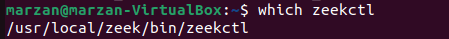
\includegraphics[width=1\linewidth]{images/live_monitor/which zeekctl.png}
    \caption{zeekctl path}
    \label{fig:enter-label}
\end{figure}

\begin{itemize}
    \item Activate the Zeek control application by executing start zeekctl, which initiates the live monitoring process.
\end{itemize}

\begin{figure}[H]
    \centering
    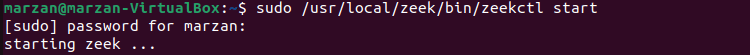
\includegraphics[width=1\linewidth]{images/live_monitor/zeetctl_start.png}
    \caption{zeekctl start}
    \label{fig:enter-label}
\end{figure}
\begin{itemize}
    \item Upon commencement of live monitoring, Zeek begins to capture and analyze network traffic, systematically storing the results in a series of log files. These logs, encompassing various protocols and activities, include but are not limited to dns.log, http.log, and dhcp.log.
\end{itemize}

\begin{figure}[H]
    \centering
    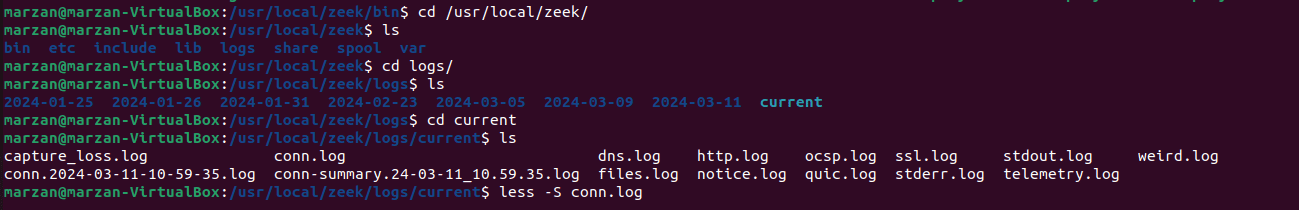
\includegraphics[width=1\linewidth]{images/live_monitor/live_logs.png}
    \caption{Log files}
    \label{fig:enter-label}
\end{figure}

\begin{itemize}
    \item To examine the connection log (conn.log), the command less -S conn.log is employed. This command provides a paginated view of the conn.log file, allowing for detailed inspection of recorded network connections.
\end{itemize}


\begin{figure}[H]
    \centering
    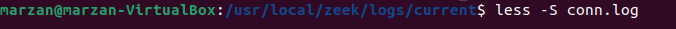
\includegraphics[width=1\linewidth]{images/live_monitor/less_conn_live.png}
    \caption{conn.log}
    \label{fig:enter-label}
\end{figure}

\begin{itemize}
    \item Further scrutiny of the conn.log file can be achieved through direct observation, facilitating a deeper understanding of the network interactions and anomalies.
\end{itemize}


\begin{figure}[H]
    \centering
    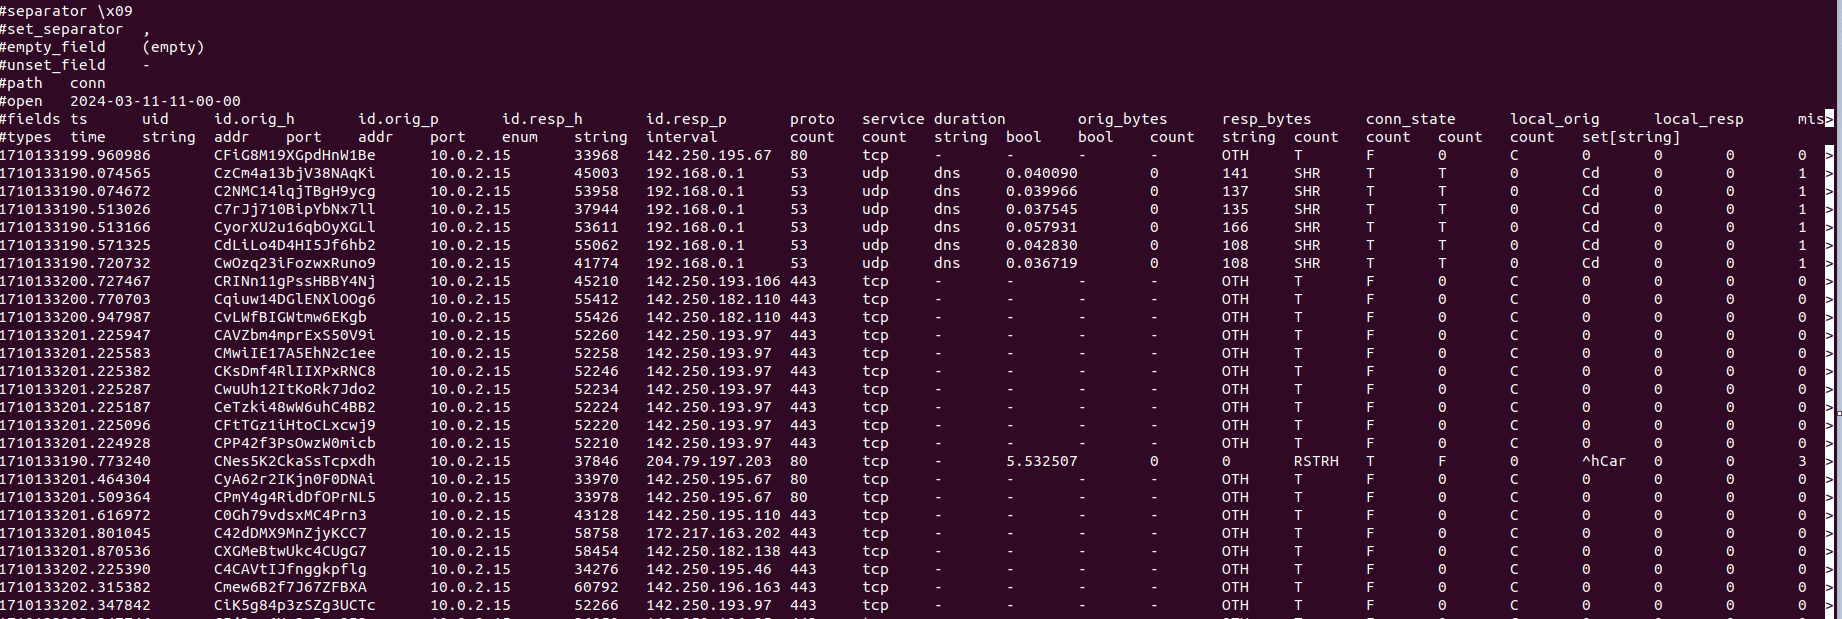
\includegraphics[width=1\linewidth]{images/new_1.png}
    \caption{conn.log}
    \label{fig:enter-label}
\end{figure}

\begin{itemize}
    \item For an enhanced analysis experience, the conn.log file may be imported into the Brim application. Brim provides a graphical interface for interacting with Zeek logs, offering advanced search capabilities and visualizations to aid in the interpretation of network data.
\end{itemize}

\begin{figure}[H]
    \centering
    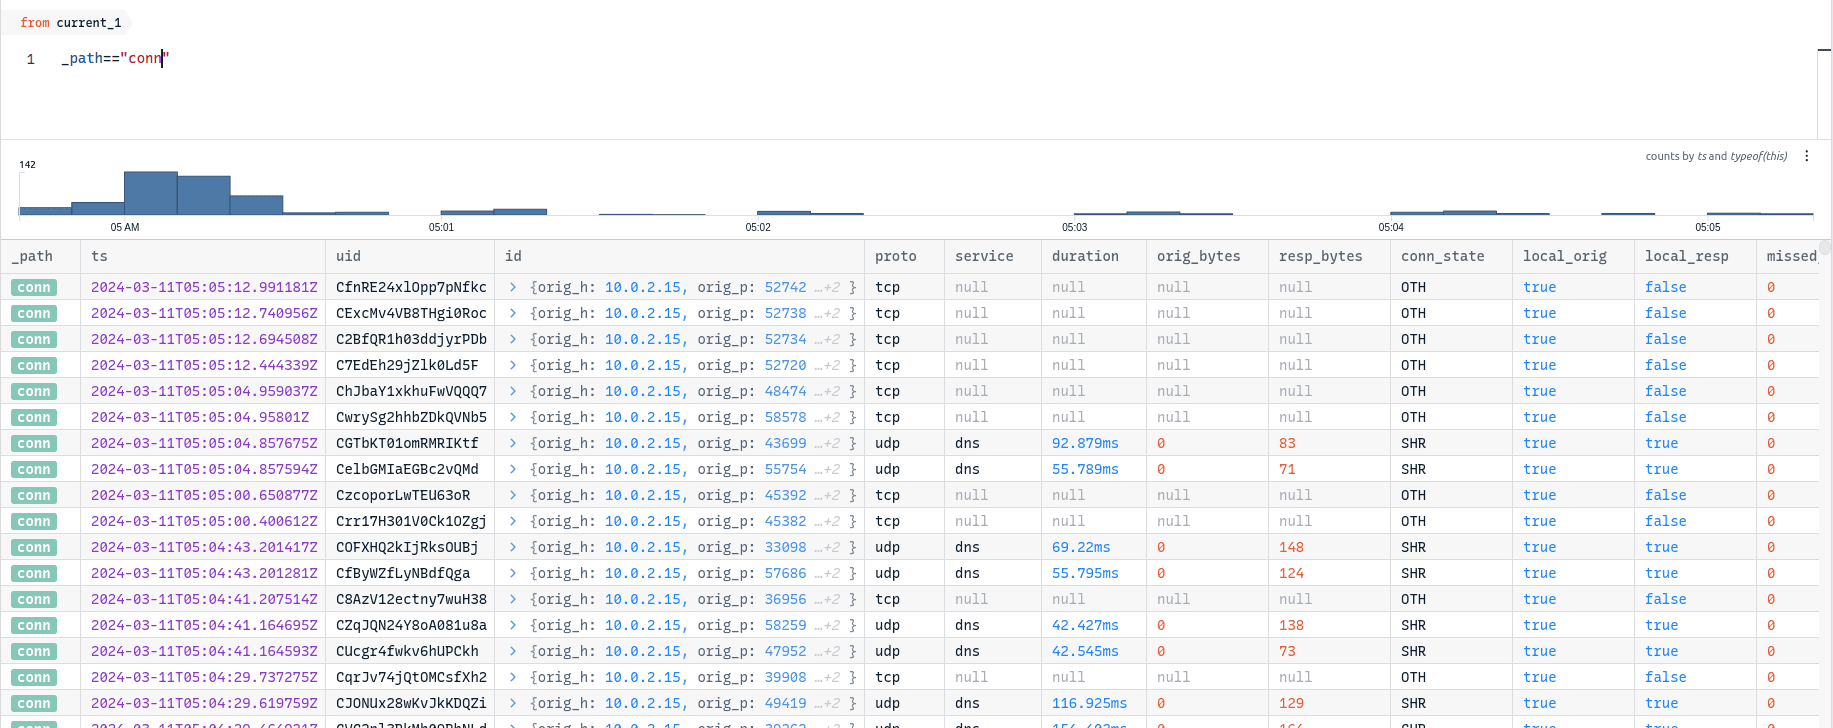
\includegraphics[width=1\linewidth]{images/live_monitor/live_brim_conn.png}
    \caption{conn.log in BRIM}
    \label{fig:enter-label}
\end{figure}

\begin{itemize}
    \item To check out the DNS activity,we have opened the dns.log file using less -S dns.log. This shows the DNS details page by page, making it easier to see what's happening.
\end{itemize}

\begin{figure}[H]
    \centering
    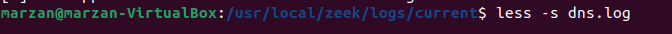
\includegraphics[width=1\linewidth]{images/live_monitor/less_dns_live.png}
    \caption{dns.log}
    \label{fig:enter-label}
\end{figure}

\begin{itemize}
    \item Direct analysis of dns.log elucidates DNS traffic patterns and anomalies.
\end{itemize}


\begin{figure}[H]
    \centering
    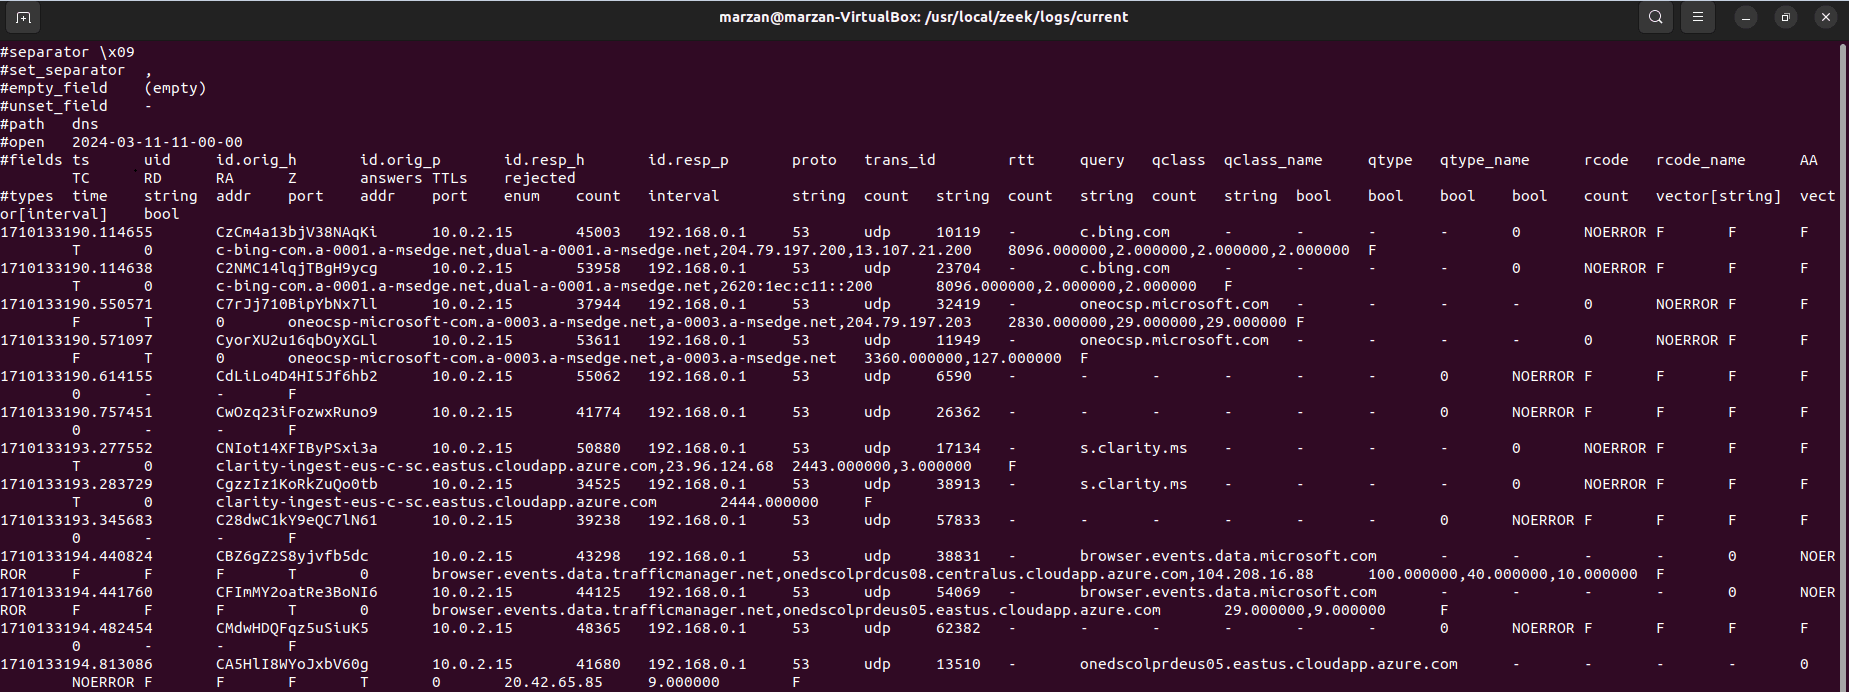
\includegraphics[width=1\linewidth]{images/new_2.png}
    \caption{dns.log}
    \label{fig:enter-label}
\end{figure}

\begin{itemize}
    \item For advanced analysis, dns.log is imported into Brim. Brim's GUI and analytical tools enhance DNS log data interpretation, offering clarity on network DNS behavior.
\end{itemize}

\begin{figure}[H]
    \centering
    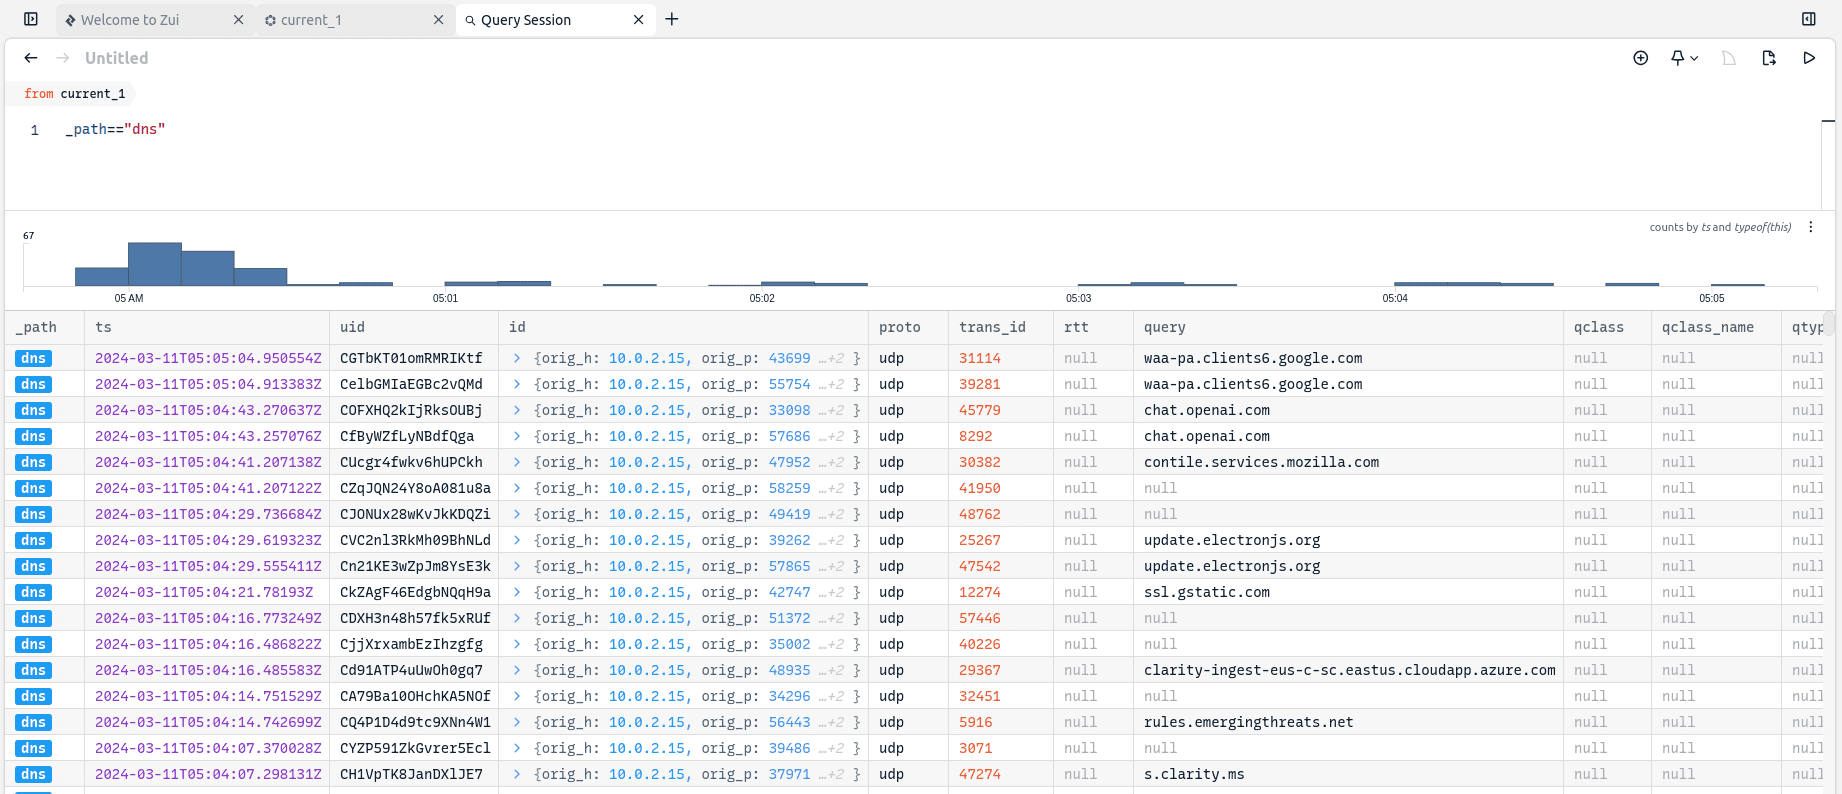
\includegraphics[width=1\linewidth]{images/live_monitor/live_brim_dns.png}
    \caption{dns.log in BRIM}
    \label{fig:enter-label}
\end{figure}



\subsection{Network Monitoring from PCAP file:}

Here is the link to PCAP file:
\href{https://www.malware-traffic-analysis.net/tutorials/index.html}{malware-traffic-analysis}\\\\

\subsubsection{Simulation :}
\begin{itemize}
    \item Begin by executing the command zeek -C -r a.pcap, which initiates the analysis of the provided PCAP file. The -C flag is used to ignore checksums, ensuring that all packets are analyzed irrespective of checksum validity.
\end{itemize}

\begin{figure}[H]
    \centering
    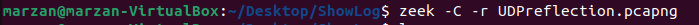
\includegraphics[width=1\linewidth]{images/pcap/pcap_1.png}
    \caption{zeek analysis of pcap file }
    \label{fig:enter-label}
\end{figure}

\begin{itemize}
    \item Upon completion of the analysis, Zeek will generate a series of log files, including but not limited to conn.log, dns.log, and weird.log, each containing detailed information pertinent to their respective network protocols and events.
\end{itemize}


\begin{figure}[H]
    \centering
    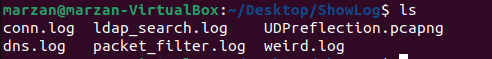
\includegraphics[width=1\linewidth]{images/pcap/pcap_2.png}
    \caption{Log files}
    \label{fig:enter-label}
\end{figure}

\begin{itemize}
    \item To review the DNS activity captured during the analysis, employ the command less -S dns.log. This command will present the contents of the dns.log file in a paginated manner, allowing for a detailed examination of DNS transactions.
\end{itemize}


\begin{figure}[H]
    \centering
    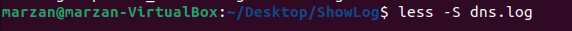
\includegraphics[width=1\linewidth]{images/pcap/pcap_4.png}
    \caption{dns.log}
    \label{fig:enter-label}
\end{figure}


\begin{figure}[H]
    \centering
    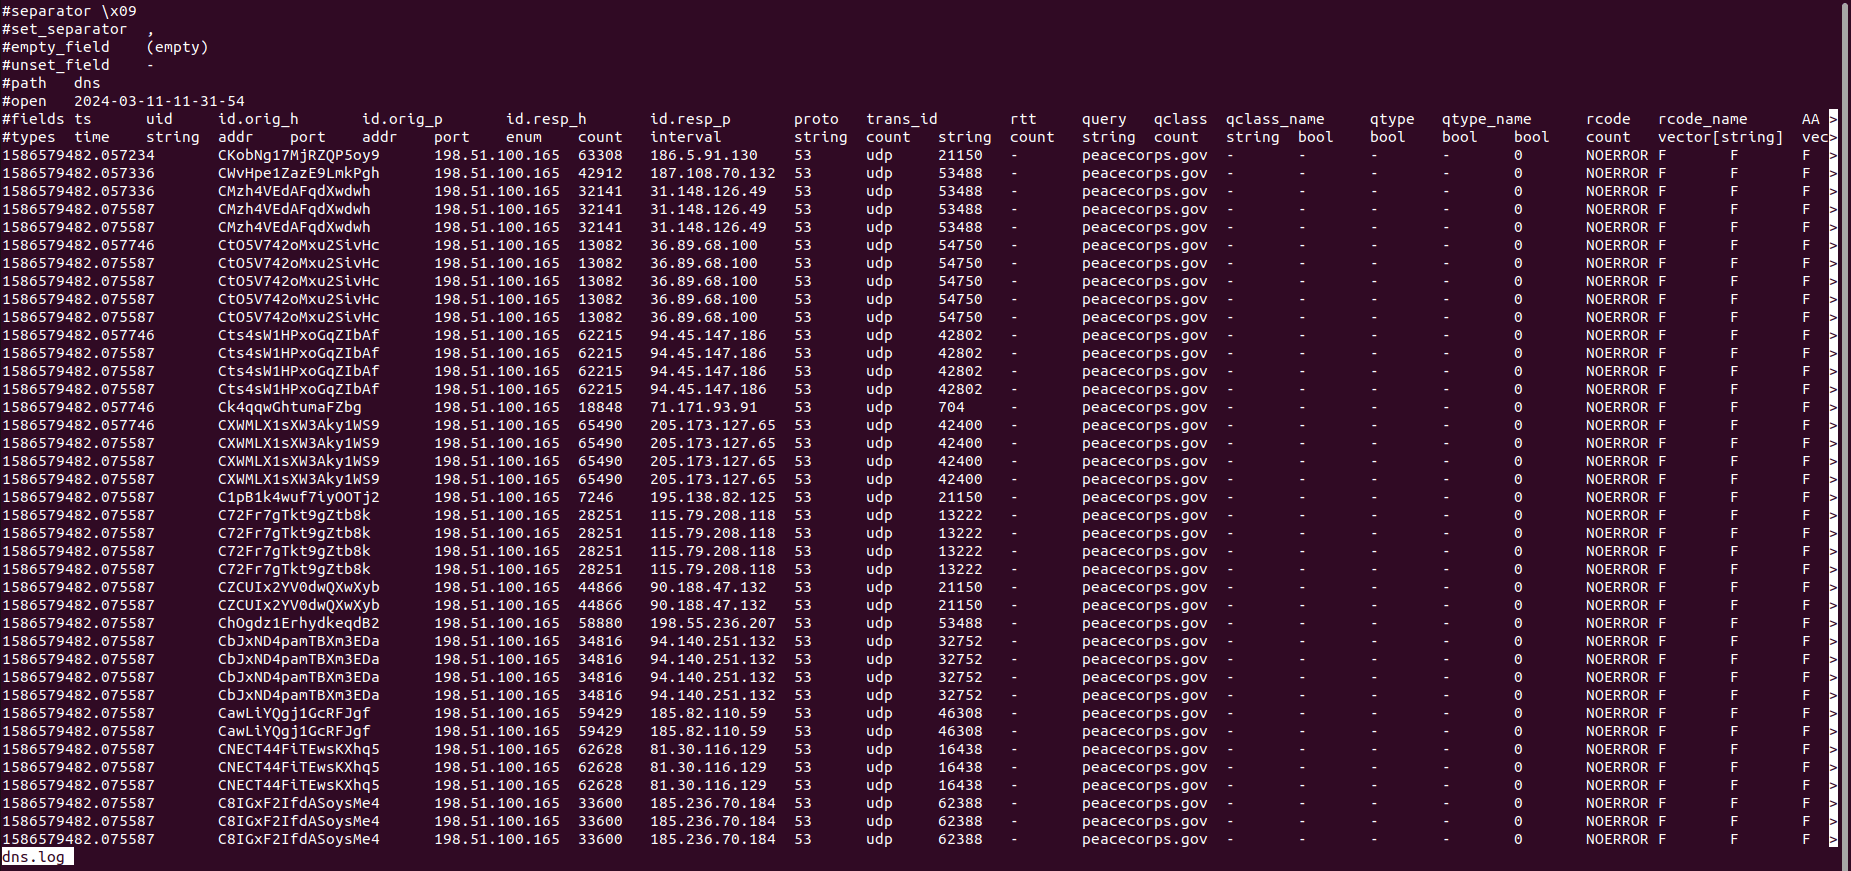
\includegraphics[width=1\linewidth]{images/pcap/pcap_3.png}
    \caption{show dns.log}
    \label{fig:enter-label}
\end{figure}

\begin{itemize}
    \item The execution of \texttt{cat dns.log | zeek-cut query | sort | uniq -c | sort -n}
 serves a critical function in aggregating and quantifying unique DNS queries. This pipeline first extracts the query field from the dns.log using zeek-cut, then sorts and counts unique instances, and finally orders them numerically.\\
    The output of the final command reveals the frequency of individual DNS queries, exemplified by 161 peacecorps.gov. This indicates that the domain peacecorps.gov was queried 161 times, highlighting it as a significant point of interest in the network traffic analyzed.
\end{itemize}


\begin{figure}[H]
    \centering
    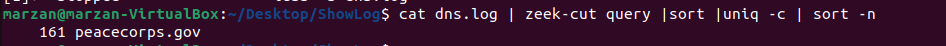
\includegraphics[width=1\linewidth]{images/pcap/pcap_5.png}
    \caption{zeek-cut for unique query}
    \label{fig:enter-label}
\end{figure}

\section{Detecting DNS Amplification Attacks with Zeek}
Zeek stands out as a powerful network security tool, capable of real-time monitoring and analysis of network traffic. It is particularly effective in detecting and mitigating DNS Amplification attacks, a type of Distributed Denial of Service (DDoS) attack that leverages public DNS servers to overwhelm a target with disproportionate DNS response traffic.
\subsection{How It Works}
The following points outline Zeek's approach to identifying DNS Amplification attacks:

\begin{enumerate}
    \item \textbf{Monitoring DNS Traffic}: Zeek meticulously observes network traffic, focusing on DNS activities to capture both query requests and their responses, thereby monitoring the exchanges between clients and DNS servers.
    
    \item \textbf{Analyzing Response Sizes}: Zeek assesses the size of DNS response packets, identifying potential amplification behavior when response sizes significantly exceed those of the query requests.
    
    \item \textbf{Establishing Baseline Metrics}: Zeek establishes baseline metrics for standard DNS traffic, including typical sizes for requests and responses and normal query rates, which assists in spotting deviations that might indicate an attack.
    
    \item \textbf{Threshold Configuration}: Within Zeek's configuration, customizable thresholds are set for factors such as response size limits and query rate caps. Surpassing these thresholds may indicate a potential DNS Amplification attack.
    
    \item \textbf{Pattern Recognition}: Zeek detects patterns that align with DNS Amplification characteristics, like an unusual influx of large response packets directed at a single target or increased queries to open DNS resolvers.
    
    \item \textbf{Incident Logging and Alerts}: When Zeek identifies anomalies consistent with DNS Amplification attacks, it logs the incidents and can also be configured to issue real-time alerts, facilitating prompt intervention and attack mitigation.
\end{enumerate}
\subsection{DNS Script :}
\begin{lstlisting}[language=Python, caption=]
@load base/protocols/dns

module Notice;

export {
    redef enum Notice::Type += {DNS_Amplification_Suspected};
}
global dns_query_threshold: count = 20;
global suspicious_dns_activity: table[addr] of count = {};

event dns_request(c: connection, msg: dns_msg, query: string, qtype: count, qclass: count) {
    local src = c$id$orig_h;
    if ( src in suspicious_dns_activity ) {
        suspicious_dns_activity[src] += 1;
    } else {
        suspicious_dns_activity[src] = 1;
    }

    if ( suspicious_dns_activity[src] > dns_query_threshold ) {
        NOTICE([$note=DNS_Amplification_Suspected,
                $msg=fmt("High volume of DNS requests from %s, potential DNS Amplification.", src),
                $src=src,
                $conn=c]);
                
        delete suspicious_dns_activity[src];
    }
}

event dns_query_reply(c: connection, msg: dns_msg, query: string, qtype: count, qclass: count) {
    local src = c$id$orig_h;
    if ( src in suspicious_dns_activity ) {
        suspicious_dns_activity[src] += 1;
    } else {
        suspicious_dns_activity[src] = 1;
    }

    if ( suspicious_dns_activity[src] > dns_query_threshold ) {
        NOTICE([$note=DNS_Amplification_Suspected,
                $msg=fmt("High volume of DNS requests from %s, potential DNS Amplification.", src),
                $src=src,
                $conn=c]);
                
        delete suspicious_dns_activity[src];
    }
}
\end{lstlisting}
\subsection{DNS Script Explanation}


\begin{enumerate}
    
    \item \textbf{DNS Script Inclusion} (Line 1): The script initiates by incorporating DNS protocol analysis functionalities through `\texttt{@load base/protocols/dns}`, enabling inspection of DNS traffic.

    \item \textbf{Notice Module Extension} (Lines 2-6): The script enhances the `\texttt{Notice}` module by appending a new notice type called `\texttt{DNS\_Amplification\_Suspected}`, designed for alerting upon detection of suspicious DNS activities.

    \item \textbf{Global Variables Declaration} (Lines 8-9):
    \begin{itemize}
        \item `\texttt{dns\_query\_threshold}`: Sets a threshold (20 in this context) to delineate the normal count of DNS queries from a single IP before it is deemed suspicious.
        \item `\texttt{suspicious\_dns\_activity}`: Initializes a table to record the number of DNS queries made by each source IP address, facilitating the tracking of DNS request frequencies.
    \end{itemize}

    \item \textbf{DNS Request Event Handling} (\texttt{dns\_request})(Lines 11-27):
    \begin{itemize}
        \item The script monitors `\texttt{dns\_request}` events, triggered by DNS queries.
        \item Extracts the source IP (`\texttt{src}`) from each DNS request's connection details.
        \item Updates the `\texttt{suspicious\_dns\_activity}` table with the query count for the source IP, adding the IP with a count of 1 if it's not already present.
        \item Generates a `\texttt{DNS\_Amplification\_Suspected}` notice if the query count for a source IP surpasses the `\texttt{dns\_query\_threshold}`, indicating potential DNS amplification attack behavior.
        \item Resets the query count for the source IP in the `\texttt{suspicious\_dns\_activity}` table by removing its entry post-notice generation to avoid repetitive alerts.
    \end{itemize}


  \item \textbf{DNS Query Reply Event (\texttt{dns\_query\_reply})  (Lines 29-45):}
  \begin{itemize}
    \item Triggered for each DNS query reply observed in the monitored traffic.
    \item Increments a counter in \texttt{suspicious\_dns\_activity} for the source IP address of the query (\texttt{c\$id\$orig\_h}).
    \item If the count for an IP address exceeds \texttt{dns\_query\_threshold}, a \texttt{DNS\_Amplification\_Suspected} notice is generated, indicating potential amplification activity from that IP address.
    \item The entry for the IP address in \texttt{suspicious\_dns\_activity} is deleted after generating the notice, resetting its count.
  \end{itemize}


\end{enumerate}


\subsection{Simulation :}
Here is the link to PCAP file:
\href{https://www.malware-traffic-analysis.net/tutorials/index.html}{malware-traffic-analysis}\\\\
\begin{itemize}
    \item The process starts by analyzing a PCAP file with dns.zeek, which uses DNS protocol analysis to detect potential DNS Amplification attacks by identifying abnormal DNS query volumes, defining a specific notice type DNS\_Amplification\_Suspected for such events.
\end{itemize}

\begin{figure}[H]
    \centering
    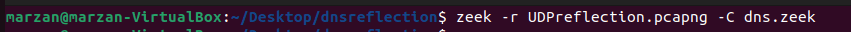
\includegraphics[width=1\linewidth]{images//UDP_reflection/udp_3.png}
    \caption{Script Execution}
    \label{fig:enter-label}
\end{figure}

\begin{itemize}
    \item The notice.log entries indicate the IP 198.51.100.165's excessive DNS requests, suggesting potential DNS Amplification attacks. These entries document the incident details, including the involved IPs and ports, and mark each event for logging with a one-hour suppression to mitigate repeat alerts.
\end{itemize}
\begin{figure}[H]
    \centering
    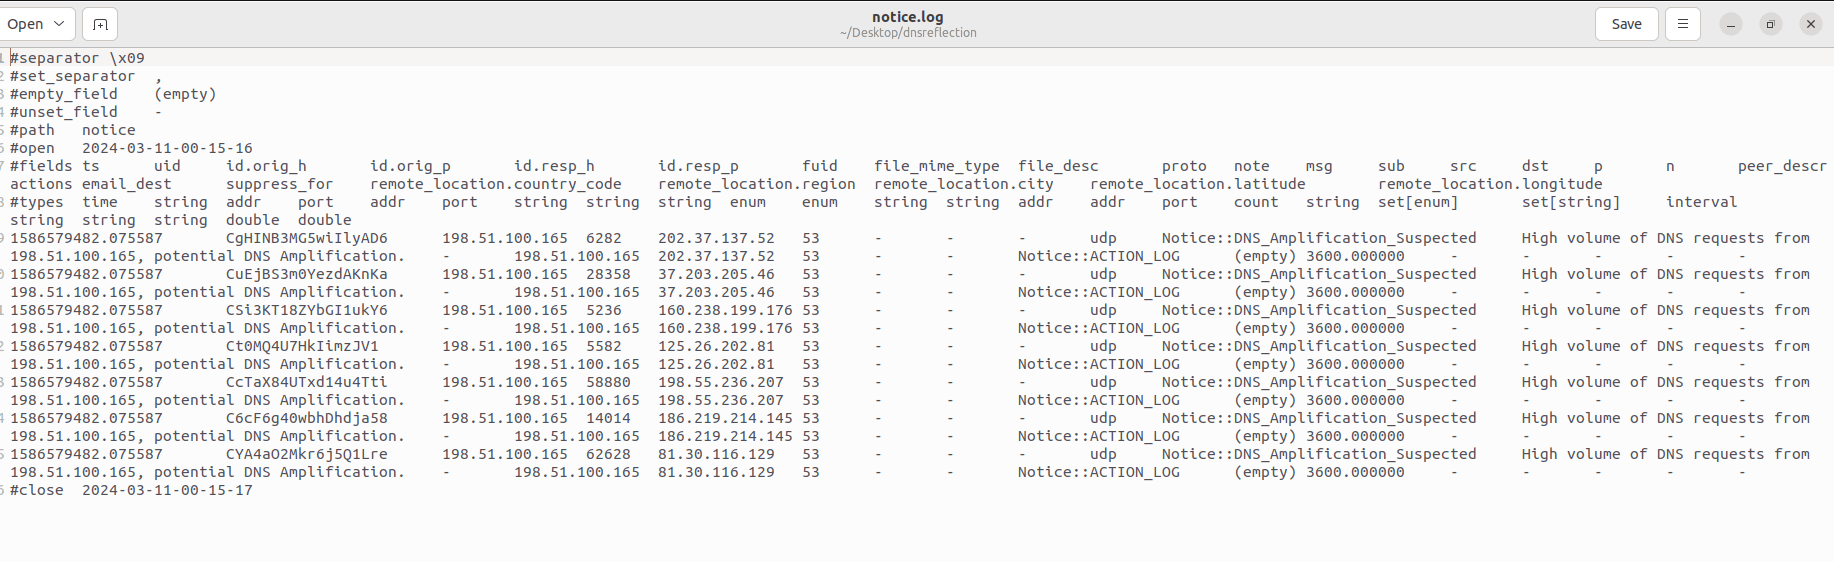
\includegraphics[width=1\linewidth]{images//UDP_reflection/udp_4.png}
    \caption{notice.log}
    \label{fig:enter-label}
\end{figure}

\begin{itemize}
    \item In BRIM, the notice.log is organized into a formal tabular representation, systematically displaying instances of potential DNS Amplification attacks originating from the IP 198.51.100.165.
\end{itemize}
\begin{figure}[H]
    \centering
    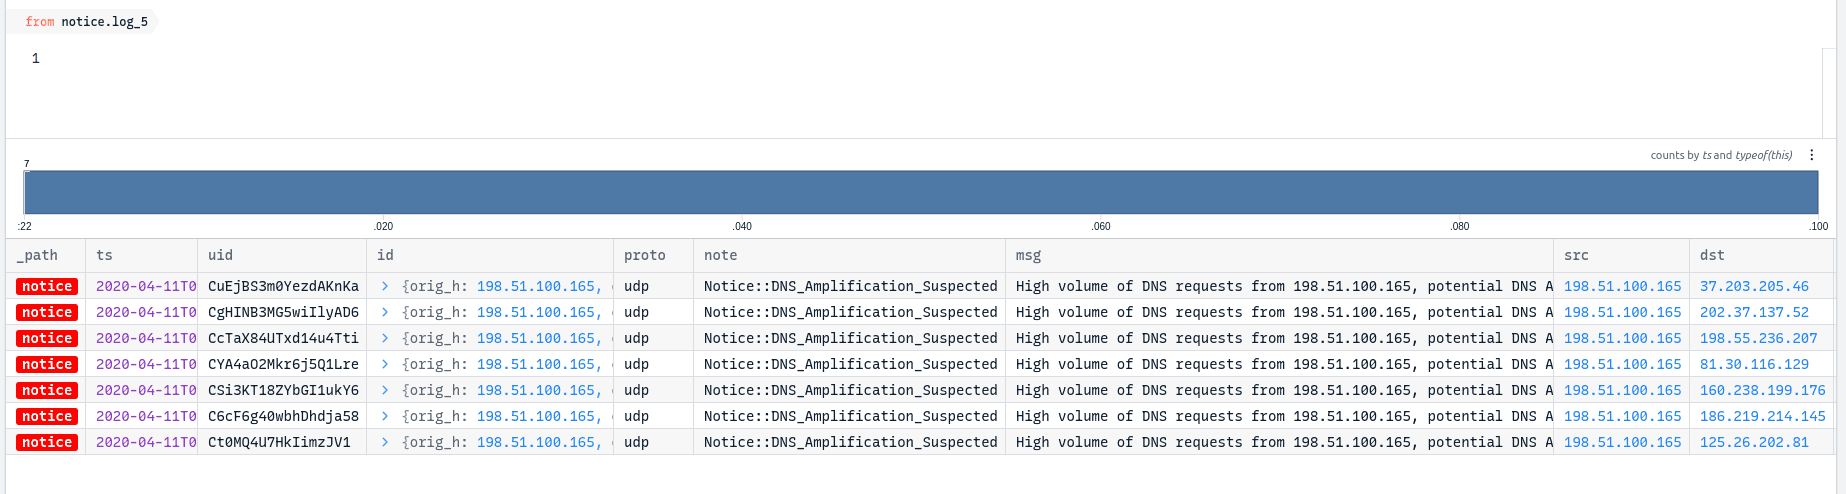
\includegraphics[width=0.8\linewidth]{images//UDP_reflection/udp_5.png}
    \caption{notice.log in BRIM}
    \label{fig:enter-label}
\end{figure}






\subsection{Example Script :}
\begin{lstlisting}[language=Python, caption=]
module DDosAttacks;
@load base/protocols/dns

redef enum Notice::Type += {
    DNSDDoSAmplification
};

function generate_ddos_notice(c: connection, query: string) {
    local query1: string = strip(query);
    if (query1 == "peacecorps.gov" || query1 == "pizzaseo.com") {
        NOTICE([$note = DNSDDoSAmplification,
            $msg = fmt("Possible DNS DDoS Amplification Attack"),
            $conn = c,
            $uid = c$uid
        ]);
    }
}

event dns_request(c: connection, msg: dns_msg, query: string, qtype: count, qclass: count, original_query: string) {
    generate_ddos_notice(c, query);
}

event dns_query_reply(c: connection, msg: dns_msg, query: string, qtype: count, qclass: count, original_query: string) {
    generate_ddos_notice(c, query);
}
\end{lstlisting}

\subsection{Example Script Explanation}

\begin{enumerate}
    
    \item \textbf{Module Declaration and DNS Script Loading} (Lines 1-2): The script commences with the declaration of a module titled `DDosAttacks`. It proceeds to integrate DNS protocol analysis functionalities from the Zeek standard library through the command `\texttt{@load base/protocols/dns}`.

    \item \textbf{Enumeration Extension for Notice} (Lines 4-5): The script enhances the `\texttt{Notice::Type}` enumeration by appending a novel type named `DNSDDoSAmplification`. This addition is aimed at facilitating the signaling of potential DNS DDoS amplification attacks.

    \item \textbf{DDoS Notice Generation Function} (Lines 8-17): A function named `\texttt{generate\_ddos\_notice}` is introduced. It is designed to examine network connections (denoted as `c`) and DNS queries (denoted as `query`). The function scrutinizes the DNS query after removing any whitespace and, if it matches specific domains (`peacecorps.gov` or `pizzaseo.com`), it issues a notice of type `DNSDDoSAmplification`.

    \item \textbf{DNS Request Event Handling} (Lines 19-21): The script configures an event handler named `\texttt{dns\_request}`. This handler is triggered for every DNS request and it invokes the `\texttt{generate\_ddos\_notice}` function. This mechanism is employed to assess each DNS inquiry for indications of DNS DDoS amplification attacks.

    \item \textbf{DNS Query Reply Event Handling} (Lines 23-25): Similarly, the script sets up another event handler named `\texttt{dns\_query\_reply}`. This handler also calls the `\texttt{generate\_ddos\_notice}` function for DNS responses, thereby extending the surveillance to include reply messages which might be pertinent in detecting attack patterns.
\end{enumerate}

\subsection{Simulation :}
Here is the link to PCAP file:
\href{https://www.malware-traffic-analysis.net/tutorials/index.html}{malware-traffic-analysis}\\\\
\begin{itemize}
    \item  The process begins with the execution of a PCAP file through the example.zeek script, part of the DDosAttacks module, which loads DNS protocol analyses. The script is designed to identify potential DNS DDoS Amplification attacks by inspecting DNS queries. If a query matches specific target domains, it triggers a DNSDDoSAmplification notice.
\end{itemize}
\begin{figure}[H]
    \centering
    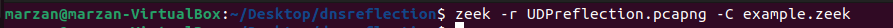
\includegraphics[width=1\linewidth]{images//UDP_reflection/udp_1.png}
    \caption{Script Execution}
    \label{fig:enter-label}
\end{figure}

\begin{itemize}
    \item The resulting notice.log entries, visualized in BRIM in a tabular format, detail instances where the script detected potential DNS DDoS Amplification attacks. Each entry includes the timestamp, source and destination IP addresses and ports, protocol used (UDP), and a message indicating a "Possible DNS DDoS Amplification Attack". The action logged is Notice::ACTION\_LOG, and a suppression period of 3600 seconds is set to prevent immediate duplicate alerts.
\end{itemize}
\begin{figure}[H]
    \centering
    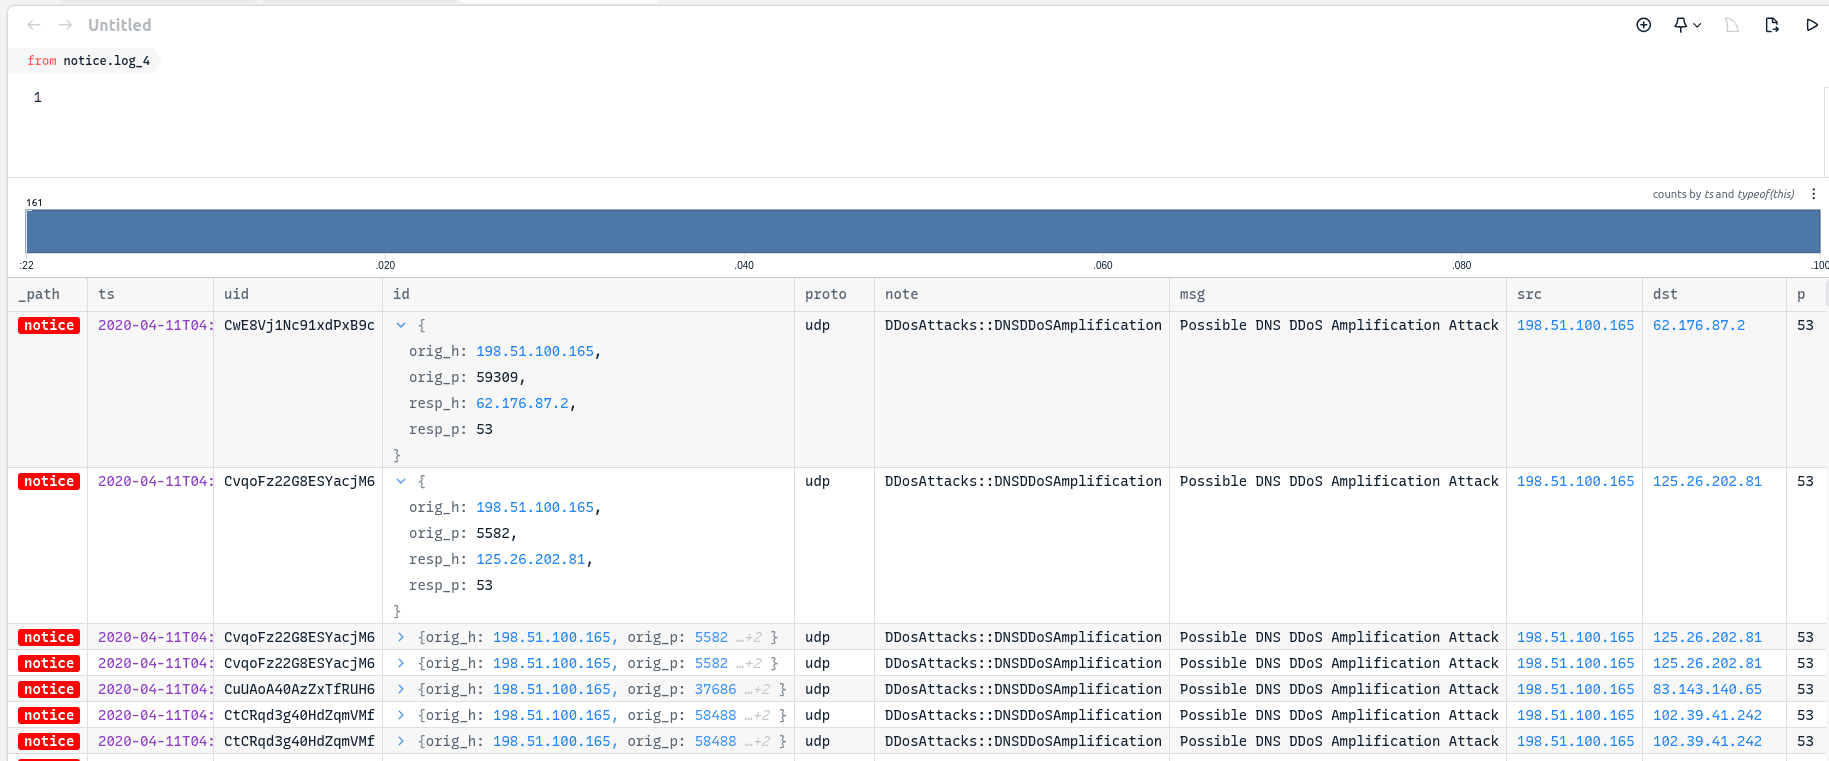
\includegraphics[width=1\linewidth]{images//UDP_reflection/udp_2.png}
    \caption{notice.log Analysis in BRIM}
    \label{fig:enter-label}
\end{figure}


\section{Detecting SSH Brute Forcing with Zeek}
Zeek is a powerful network traffic analyzer that plays a crucial role in cybersecurity defenses by monitoring and analyzing network traffic in real time. It's particularly adept at identifying and mitigating security threats, such as SSH brute force attacks. An SSH brute force attack involves an attacker attempting numerous passwords or passphrase combinations to gain unauthorized access to a system. Zeek's approach to detecting such attacks hinges on its ability to scrutinize the intricacies of SSH traffic, focusing on the authentication process.

\subsection{How It Works}
Here's a concise breakdown of how Zeek detects SSH brute forcing:

\begin{enumerate}
    \item \textbf{Monitoring SSH Traffic:} Zeek listens to network traffic, focusing on the SSH protocol to capture the initial handshake, authentication attempts, and the session's lifecycle.
    \item \textbf{Analyzing Authentication Responses:} It examines the size of the server's response packets post-authentication attempts. A response size around 5k bytes often signifies a successful login, which Zeek uses as a heuristic measure.
    \item \textbf{Setting Detection Thresholds:} Parameters like ``password\_guesses\_limit'' and ``guessing\_timeout'' within Zeek's SSH brute forcing script help define the acceptable number of failed login attempts within a certain timeframe, beyond which an attack is presumed.
    \item \textbf{Identifying Brute Force Patterns:} Zeek flags a sequence of failed logins (indicated by ``auth\_success'' set to ``F'') exceeding the predefined threshold within the set timeframe as a brute force attempt.
    \item \textbf{Logging and Alerting:} Following the detection of a brute force attack, Zeek logs the event and can generate alerts, facilitating prompt investigation and response.
\end{enumerate}

\subsection{Detect-bruteforcing.zeek Script:}



\begin{lstlisting}[language=Python, caption=detect-bruteforcing.zeek]
##! Detect hosts which are doing password guessing attacks and/or password
##! bruteforcing over SSH.

@load base/protocols/ssh
@load base/frameworks/sumstats
@load base/frameworks/notice
@load base/frameworks/intel
module SSH;
export {
	redef enum Notice::Type += {
		## Indicates that a host has been identified as crossing the
		## :zeek:id:`SSH::password_guesses_limit` threshold with
		## failed logins.
		Password_Guessing,
		## Indicates that a host previously identified as a "password
		## guesser" has now had a successful login
		## attempt. This is not currently implemented.
		Login_By_Password_Guesser,
	};

	redef enum Intel::Where += {
		## An indicator of the login for the intel framework.
		SSH::SUCCESSFUL_LOGIN,
	};

	## The number of failed SSH connections before a host is designated as
	## guessing passwords.
	const password_guesses_limit: double = 30 &redef;

	## The amount of time to remember presumed non-successful logins to
	## build a model of a password guesser.
	const guessing_timeout = 30 mins &redef;

	## This value can be used to exclude hosts or entire networks from being
	## tracked as potential "guessers". The index represents
	## client subnets and the yield value represents server subnets.
	const ignore_guessers: table[subnet] of subnet &redef;
}

event zeek_init()
	{
	local r1: SumStats::Reducer = [$stream="ssh.login.failure", $apply=set(SumStats::SUM, SumStats::SAMPLE), $num_samples=5];
	SumStats::create([$name="detect-ssh-bruteforcing",
	                  $epoch=guessing_timeout,
	                  $reducers=set(r1),
	                  $threshold_val(key: SumStats::Key, result: SumStats::Result) =
	                  	{
	                  	return result["ssh.login.failure"]$sum;
	                  	},
	                  $threshold=password_guesses_limit,
	                  $threshold_crossed(key: SumStats::Key, result: SumStats::Result) =
	                  	{
	                  	local r = result["ssh.login.failure"];
	                  	local sub_msg = fmt("Sampled servers: ");
	                  	local samples = r$samples;
	                  	for ( i in samples )
	                  		{
	                  		if ( samples[i]?$str )
	                  			sub_msg = fmt("%s%s %s", sub_msg, i==0 ? "":",", samples[i]$str);
	                  		}
	                  	# Generate the notice.
	                  	NOTICE([$note=Password_Guessing,
	                  	        $msg=fmt("%s appears to be guessing SSH passwords (seen in %d connections).", key$host, r$num),
	                  	        $sub=sub_msg,
	                  	        $src=key$host,
	                  	        $identifier=cat(key$host)]);
	                  	}]);
	}

event ssh_auth_successful(c: connection, auth_method_none: bool)
	{
	local id = c$id;

	Intel::seen([$host=id$orig_h,
	             $conn=c,
	             $where=SSH::SUCCESSFUL_LOGIN]);
	}

event ssh_auth_failed(c: connection)
	{
	local id = c$id;

	# Add data to the FAILED_LOGIN metric unless this connection should
	# be ignored.
	if ( ! (id$orig_h in ignore_guessers &&
	        id$resp_h in ignore_guessers[id$orig_h]) )
		SumStats::observe("ssh.login.failure", [$host=id$orig_h], [$str=cat(id$resp_h)]);
	}

\end{lstlisting}


\subsection{Detect-bruteforcing.zeek Script Explanation}
\begin{enumerate}
    \item \textbf{Notice Types Extension} (Lines 10-19): Extends Zeek's notice framework with `Password\_Guessing` and `Login\_By\_Password\_Guesser` for flagging SSH brute force activities and successful logins by flagged hosts.
    
    \item \textbf{Intel Framework Extension} (Lines 21-24): Adds `SSH::SUCCESSFUL\_LOGIN` to the Intel framework, tracking successful SSH logins from hosts involved in brute force activities.
    
    \item \textbf{Configuration Constants} (Lines 26-36): Sets `password\_guesses\_limit` to 30 and `guessing\_timeout` to 30 minutes, defining the threshold for failed login attempts and the time window for their evaluation.
    
    \item \textbf{SumStats Framework Integration} (Lines 38-68): Utilizes `SumStats` for aggregating failed SSH login attempts, employing a reducer with `"ssh.login.failure"` and configuring aggregation functions with a sample size of 5. Threshold evaluation and crossing logic are based on the sum of failed login attempts.
    
    \item \textbf{Successful Login Intel Reporting} (Lines 70-77): Logs successful SSH authentications through the `ssh\_auth\_successful` event using `Intel::seen`, marking with `SSH::SUCCESSFUL\_LOGIN`.
    
    \item \textbf{Failed Login Data Collection} (Lines 79-87): Captures and logs each failed SSH login attempt in the `ssh\_auth\_failed` event, excluding those from `ignore\_guessers`, contributing to brute force detection analysis.
\end{enumerate}
\subsection{SSHAttack Script :}
\begin{lstlisting}[language=Python, caption=sshAttack.zeek]
module SShAttacks;

@load protocols/ssh/detect-bruteforcing
redef SSH::password_guesses_limit=3;

hook Notice::policy(n: Notice::Info) {
  if ( n$note == SSH::Password_Guessing ) {
    add n$actions[Notice::ACTION_LOG];
  }
}

\end{lstlisting}

\subsection{SSHAttack Script Explanation}

\begin{enumerate}
    \item \textbf{Module Declaration}  (Line 1): Declares a new module \texttt{SShAttacks} for organizing script functionalities. The script's module naming might contain a capitalization typo in "SSH".
    \item \textbf{Load Statement}   (Line 3): Instructs Zeek to load the \texttt{detect-bruteforcing} script from the SSH protocol analysis suite, which contains logic for identifying potential brute force attempts.
    \item \textbf{Variable Redefinition}   (Line 4): Sets the brute force detection threshold at three failed attempts by redefining \texttt{SSH::password\_guesses\_limit} to 3.
    \item \textbf{Notice Framework Hook} (Line 6): Implements a hook into Zeek's Notice framework with \texttt{hook Notice::policy(n: Notice::Info) \{ ...\}}, allowing customized handling of notable events, particularly SSH password guessing.
    \item \textbf{Notice Handling}   (Lines 7-8): Within the hook, the script checks for notices related to SSH password guessing (\texttt{n\$note == SSH::Password\_Guessing}) and logs these events (\texttt{add n\$actions[Notice::ACTION\_LOG];}) for further analysis.
\end{enumerate}

\subsection{Simulation : }
Here is the link to PCAP file:
\href{https://www.malware-traffic-analysis.net/tutorials/index.html}{malware-traffic-analysis}\\\\
\begin{itemize}
    \item The PCAP file is executed within Zeek using the 'ssAttack.zeek' script for analysis.
\end{itemize}
\begin{figure}[H]
    \centering
    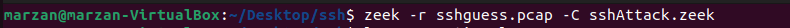
\includegraphics[width=1\linewidth]{images//UDP_reflection/ssh_1.png}
    \caption{Executing PCAP file in Zeek with 'ssAttack.zeek' script}
    \label{fig:enter-label}
\end{figure}

\begin{itemize}
    \item This notice log entry from Zeek indicates that the IP address 192.168.56.1 was detected attempting SSH password guessing, observed over three connections to 192.168.56.103. The activity triggered a SSH::Password\_Guessing alert, and the system took the action to log the event (Notice::ACTION\_LOG). An alert suppression period of one hour (3600.000000 seconds) was set following this detection.
\end{itemize}
\begin{figure}[H]
    \centering
    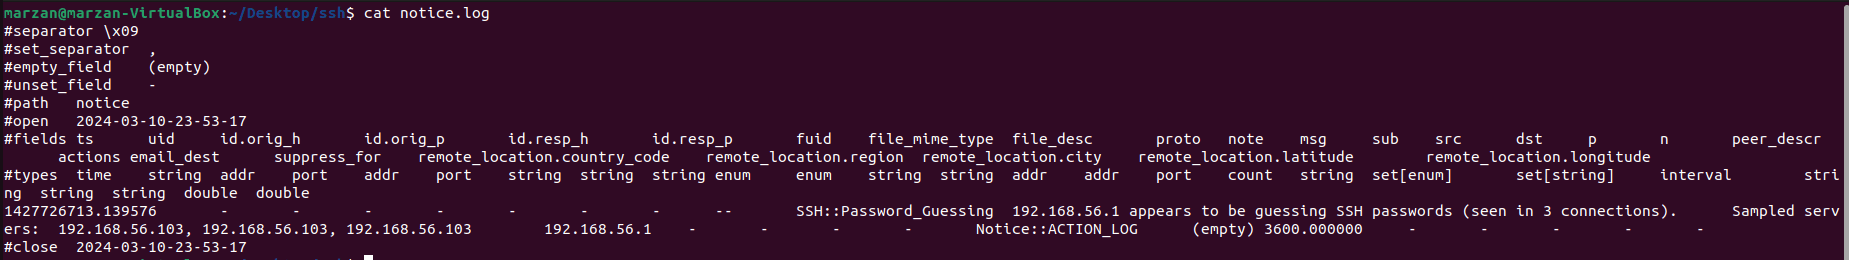
\includegraphics[width=1\linewidth]{images//UDP_reflection/ssh_2.png}
    \caption{notice.log}
    \label{fig:enter-label}
\end{figure}

\begin{itemize}
    \item In BRIM, the notice log entry is presented in a structured tabular format, detailing the detection of an SSH password guessing attempt.
\end{itemize}
\begin{figure}[H]
    \centering
    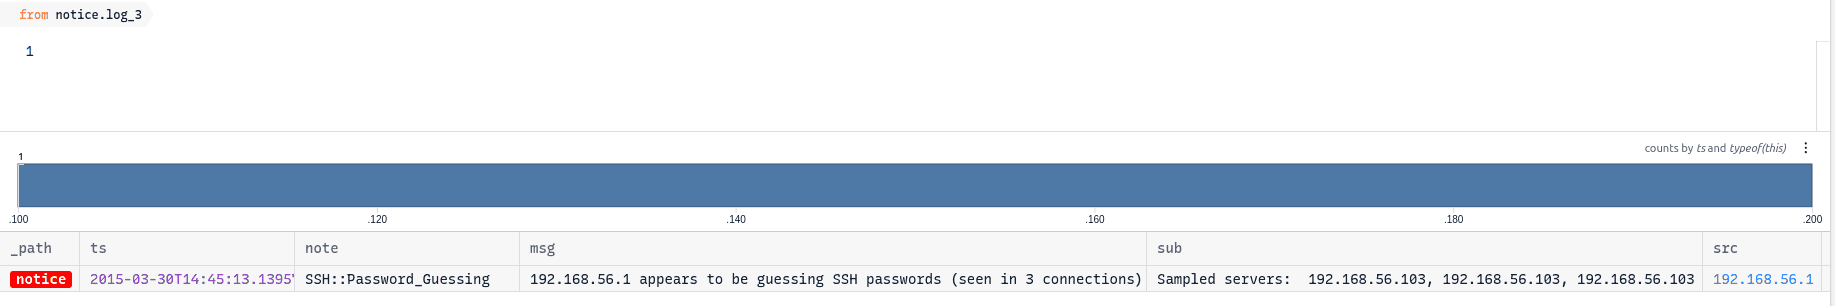
\includegraphics[width=1\linewidth]{images//UDP_reflection/ssh_3.png}
    \caption{notice.log in BRIM}
    \label{fig:enter-label}
\end{figure}



\section{JA3 Fingerprinting and Zeek Integration}
The advent of encryption in network communications, while enhancing privacy and security, has also enabled malicious actors to conceal their activities. This report details a solution to this challenge through the integration of JA3 fingerprinting with Zeek, aimed at identifying and alerting on Trickbot malware communications.
\subsection{How It Works}
The integration of JA3 fingerprinting with Zeek to detect Trickbot malware communications works through a series of coordinated steps, leveraging the unique capabilities of both technologies to identify and alert on potential security threats in encrypted network traffic. Here's a summary of how it works:

\begin{itemize}
    \item \textbf{JA3 Fingerprinting:} JA3 generates unique fingerprints for SSL/TLS clients based on TLS handshake details, creating a consistent hash value for client identification.

    \item \textbf{Custom Zeek Script:} A Zeek script is developed to capture TLS handshakes, apply JA3 hashing, and generate fingerprints for network traffic analysis.

    \item \textbf{Trickbot Hash Matching:} The script compares generated JA3 hashes against a database of known Trickbot-associated hashes to identify potential malware communications.

    \item \textbf{Detection and Alerting:} When a JA3 hash matches a known Trickbot hash, Zeek triggers an alert, signaling a potential security threat.

    \item \textbf{Logging and Analysis:} Detected events and their details are logged for further investigation, providing valuable data for incident response and threat intelligence.

    \item \textbf{Enhanced Security Posture:} Integrating JA3 with Zeek improves the detection of encrypted malware communications, enhancing the network's security monitoring capabilities.
    
\end{itemize}

\subsection{JA3 Script : }


The following listing presents the Zeek script used for JA3 fingerprinting.

\begin{lstlisting}[language=Python, caption=JA3 Fingerprinting Zeek Script]
module JA3;

export {
redef enum Log::ID += { LOG };
}

type TLSFPStorage: record {
       client_version:  count &default=0 &log;
       client_ciphers:  string &default="" &log;
       extensions:      string &default="" &log;
       e_curves:        string &default="" &log;
       ec_point_fmt:    string &default="" &log;
};
redef record connection += {
       tlsfp: TLSFPStorage &optional;
};

redef record SSL::Info += {
  ja3:            string &optional &log;
# LOG FIELD VALUES ##
#  ja3_version:  string &optional &log;
#  ja3_ciphers:  string &optional &log;
#  ja3_extensions: string &optional &log;
#  ja3_ec:         string &optional &log;
#  ja3_ec_fmt:     string &optional &log;
};

# Google. https://tools.ietf.org/html/draft-davidben-tls-grease-01

const grease: set[int] = {
    2570, 6682, 10794, 14906, 19018, 23130, 27242, 31354, 35466, 39578, 43690, 47802, 51914, 56026, 60138, 64250
};

const sep = "-";
event zeek_init() {

    Log::create_stream(JA3::LOG,[$columns=TLSFPStorage, $path="tlsfp"]);
}

event ssl_extension(c: connection, is_orig: bool, code: count, val: string)
{
    if ( is_orig == T ) {
        if ( code in grease ) {
            return;
        }
        if ( ! c?$tlsfp ){
            c$tlsfp=TLSFPStorage();
        }
        if ( c$tlsfp$extensions == "" ) {
            c$tlsfp$extensions = cat(code);
        }
        else {
            c$tlsfp$extensions = string_cat(c$tlsfp$extensions, sep,cat(code));
        }
    }
}

event ssl_extension_ec_point_formats(c: connection, is_orig: bool, point_formats: index_vec)
{
    if ( is_orig == T ) {
        if ( !c?$tlsfp )
            c$tlsfp=TLSFPStorage();
        for ( i in point_formats ) {
            if ( point_formats[i] in grease ) {
            next;
            }
            if ( c$tlsfp$ec_point_fmt == "" ) {
            c$tlsfp$ec_point_fmt += cat(point_formats[i]);
            }
            else {
            c$tlsfp$ec_point_fmt += string_cat(sep,cat(point_formats[i]));
            }
        }
    }
}

event ssl_extension_elliptic_curves(c: connection, is_orig: bool, curves: index_vec)
{
    if ( !c?$tlsfp )
    c$tlsfp=TLSFPStorage();
    if ( is_orig == T  ) {
        for ( i in curves ) {
            if ( curves[i] in grease ) {
            next;
            }
            if ( c$tlsfp$e_curves == "" ) {
             c$tlsfp$e_curves += cat(curves[i]);
            }
            else {
                c$tlsfp$e_curves += string_cat(sep,cat(curves[i]));
            }
        }
   }
}

@if ( ( Version::number >= 20600 ) || ( Version::number == 20500 && Version::info$commit >= 944 ) )
event ssl_client_hello(c: connection, version: count, record_version: count, possible_ts: time, client_random: string, session_id: string, ciphers: index_vec, comp_methods: index_vec) &priority=1
@else
event ssl_client_hello(c: connection, version: count, possible_ts: time, client_random: string, session_id: string, ciphers: index_vec) &priority=1
@endif
{
    if ( !c?$tlsfp )

    c$tlsfp=TLSFPStorage();

    c$tlsfp$client_version = version;

    for ( i in ciphers ) {

        if ( ciphers[i] in grease ) {
            next;
        }
        if ( c$tlsfp$client_ciphers == "" ) { 
            c$tlsfp$client_ciphers += cat(ciphers[i]);
        }
        else {
            c$tlsfp$client_ciphers += string_cat(sep,cat(ciphers[i]));
        }
    }
    local sep2 = ",";
    local ja3_string = string_cat(cat(c$tlsfp$client_version),sep2,c$tlsfp$client_ciphers,sep2,c$tlsfp$extensions,sep2,c$tlsfp$e_curves,sep2,c$tlsfp$ec_point_fmt);
    local tlsfp_1 = md5_hash(ja3_string);
    c$ssl$ja3 = tlsfp_1;

# LOG FIELD VALUES ##
#c$ssl$ja3_version = cat(c$tlsfp$client_version);
#c$ssl$ja3_ciphers = c$tlsfp$client_ciphers;
#c$ssl$ja3_extensions = c$tlsfp$extensions;
#c$ssl$ja3_ec = c$tlsfp$e_curves;
#c$ssl$ja3_ec_fmt = c$tlsfp$ec_point_fmt;

#
# FOR DEBUGGING ##
#print "JA3: "+tlsfp_1+" Fingerprint String: "+ja3_string;

}
\end{lstlisting}

\subsection{JA3 Script Explanation}
\begin{enumerate}
    \item \textbf{Module Initialization:} The script declares a `JA3` module and extends Zeek's logging capabilities to include JA3 fingerprints.
    
    \item \textbf{Data Structures:}
    \begin{enumerate}
        \item \textbf{TLSFPStorage:} A record that stores TLS handshake components such as the TLS version, cipher suites, SSL extensions, elliptic curves, and EC point formats.
        \item The Zeek `connection` record is extended to include a `tlsfp` field for storing TLS fingerprint data.
    \end{enumerate}
    
    \item \textbf{SSL::Info Extension:} The `SSL::Info` record is augmented with a `ja3` field to hold the MD5 hash of the JA3 fingerprint.
    
    \item \textbf{GREASE Handling:} The script accounts for GREASE values in the TLS handshake, ensuring they are ignored to maintain fingerprint integrity.
    
    \item \textbf{Event Handlers:}
    \begin{enumerate}
        \item \textbf{ssl\_extension:} Captures SSL extensions, excluding GREASE values, for JA3 string construction.
        \item \textbf{ssl\_extension\_ec\_point\_formats} and \textbf{ssl\_extension\_elliptic\_curves:} Manage elliptic curve information critical for JA3 fingerprinting.
        \item \textbf{ssl\_client\_hello:} Processes the client's initial handshake message, extracting key information to assemble the JA3 string, which is then hashed to produce the JA3 fingerprint.
    \end{enumerate}
    
    \item \textbf{JA3 Hash Generation:} The JA3 string, a concatenation of selected handshake properties, is hashed using MD5 to generate the fingerprint, uniquely identifying SSL/TLS clients.
\end{enumerate}


\subsection{Notice Script:}

\begin{lstlisting}[language=Python, caption=JA3 notice.zeek]
@load base/frameworks/notice
module JA3;

redef enum Notice::Type += {
    TrickBotDetection
};

export {
    global target_ja3_hash = "6734f37431670b3ab4292b8f60f29984"; 
}


event ssl_client_hello(c: connection, version: count, record_version: count, possible_ts: time, client_random: string, session_id: string, ciphers: index_vec, comp_methods: index_vec) &priority=1
{
    if (c$ssl$ja3 == target_ja3_hash) {
        local msg = fmt("Detected target JA3 hash (%s) for connection: %s (Orig: %s, Resp: %s)", target_ja3_hash, c$id, c$id$orig_h, c$id$resp_h);
        NOTICE([$note=TrickBotDetection, $msg=msg, $src=c$id$orig_h, $dst=c$id$resp_h]);
    }
}

\end{lstlisting}

\subsection{Notice Script Explanation}
\begin{enumerate}
    \item \textbf{Notice Framework Integration}: Utilizes Zeek's \texttt{base/frameworks/notice} module for alert generation.
    \item \textbf{JA3 Module Declaration}: Establishes a JA3 module to encapsulate JA3 hashing logic.
    \item \textbf{Notice Type Extension}: Introduces \texttt{TrickBotDetection} as a new notice type for specific categorization of alerts.
    \item \textbf{Target JA3 Hash Definition}: Sets \texttt{target\_ja3\_hash} with the JA3 hash signature of Trickbot malware for comparison.
    \item \textbf{SSL Client Hello Analysis}: 
        \begin{enumerate}
            \item Extracts parameters from \texttt{ssl\_client\_hello} messages necessary for JA3 hash computation.
            \item Computes the JA3 hash based on these parameters.
        \end{enumerate}
    \item \textbf{Detection and Alerting}:
        \begin{enumerate}
            \item Compares the computed JA3 hash with the \texttt{target\_ja3\_hash}.
            \item Generates a \texttt{TrickBotDetection} notice upon hash match, indicating potential Trickbot activity.
        \end{enumerate}
\end{enumerate}

\subsection {Simulation}

Here is the link to PCAP file:
\href{https://www.malware-traffic-analysis.net/tutorials/index.html}{malware-traffic-analysis}\\\\

\begin{itemize}
    \item The PCAP file is processed using ja3.zeek and notice.zeek scripts in Zeek. The ja3.zeek script generates JA3 hashes for TLS handshakes, while notice.zeek identifies hashes matching Trickbot signatures, creating alerts in notice.log.
\end{itemize}

\begin{figure}[H]
    \centering
    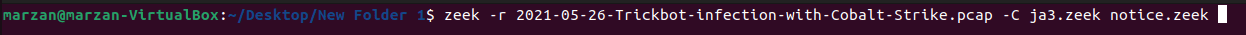
\includegraphics[width=1\linewidth]{images//ja3image/21.PNG}
    \caption{run pcap file with ja3.zeek and notice.zeek script}
    \label{fig:enter-label}
\end{figure}

\begin{itemize}
    \item The ssl.log file is examined to review detailed TLS handshake records and associated JA3 hashes generated during the simulation.
\end{itemize}
\begin{figure}[H]
    \centering
    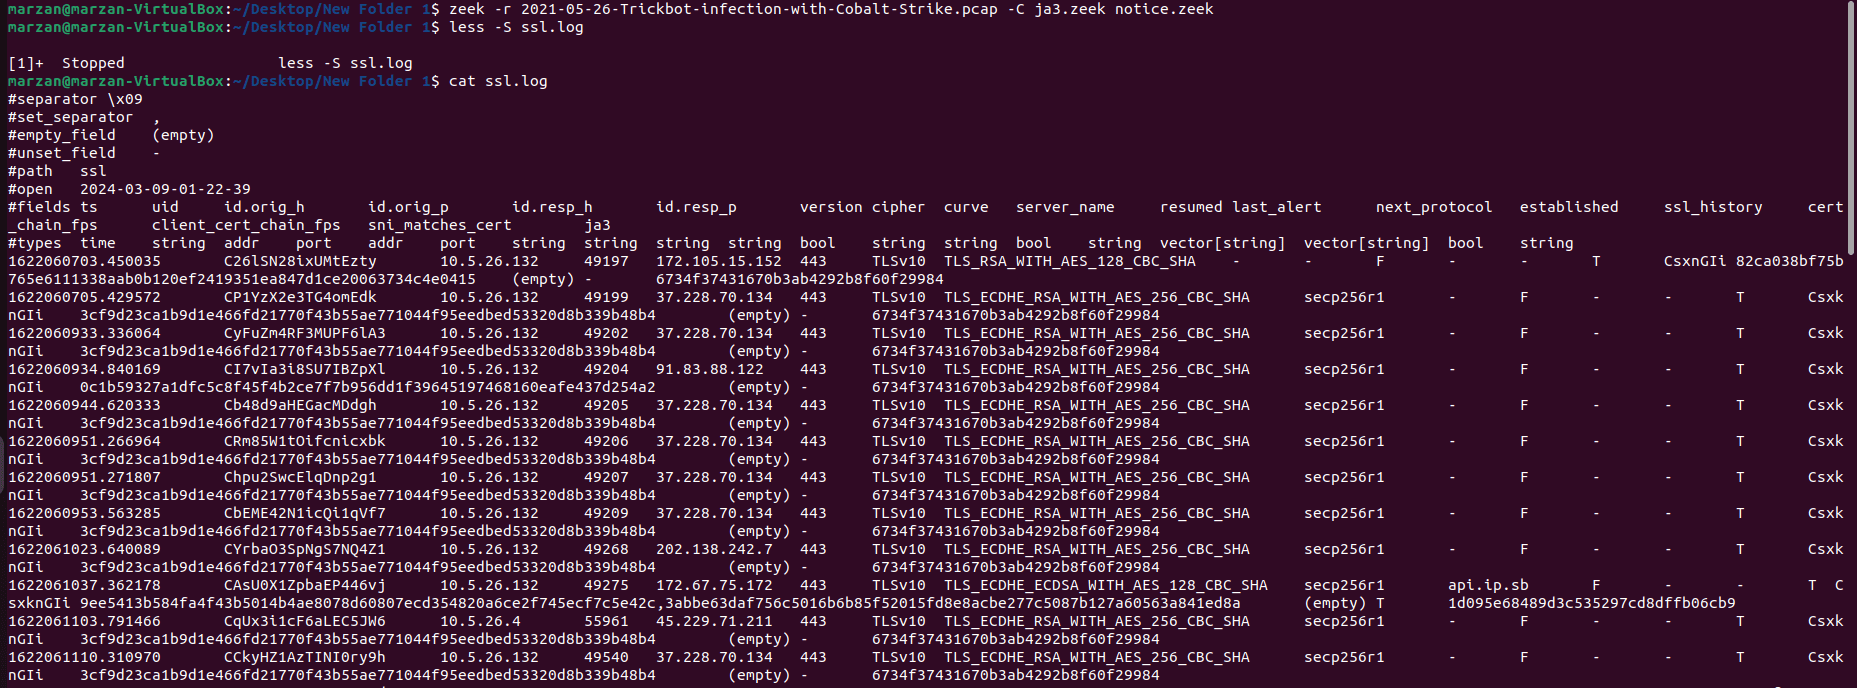
\includegraphics[width=1\linewidth]{images//ja3image/22.PNG}
    \caption{ssl.log}
    \label{fig:enter-label}
\end{figure}

\begin{itemize}
    \item Specific JA3 hash fields are extracted from the ssl.log for focused analysis.
\end{itemize}
\begin{figure}[H]
    \centering
    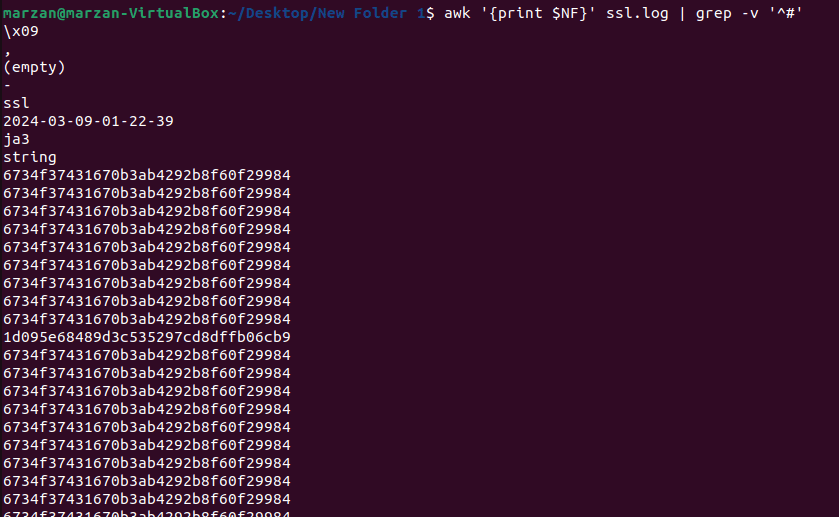
\includegraphics[width=1\linewidth]{images//ja3image/25.PNG}
    \caption{ja3 entries}
    \label{fig:enter-label}
\end{figure}

\begin{itemize}
    \item The ssl.log entries are visualized in BRIM, offering a tabular representation of SSL transactions and JA3 hashes
\end{itemize}
\begin{figure}[H]
    \centering
    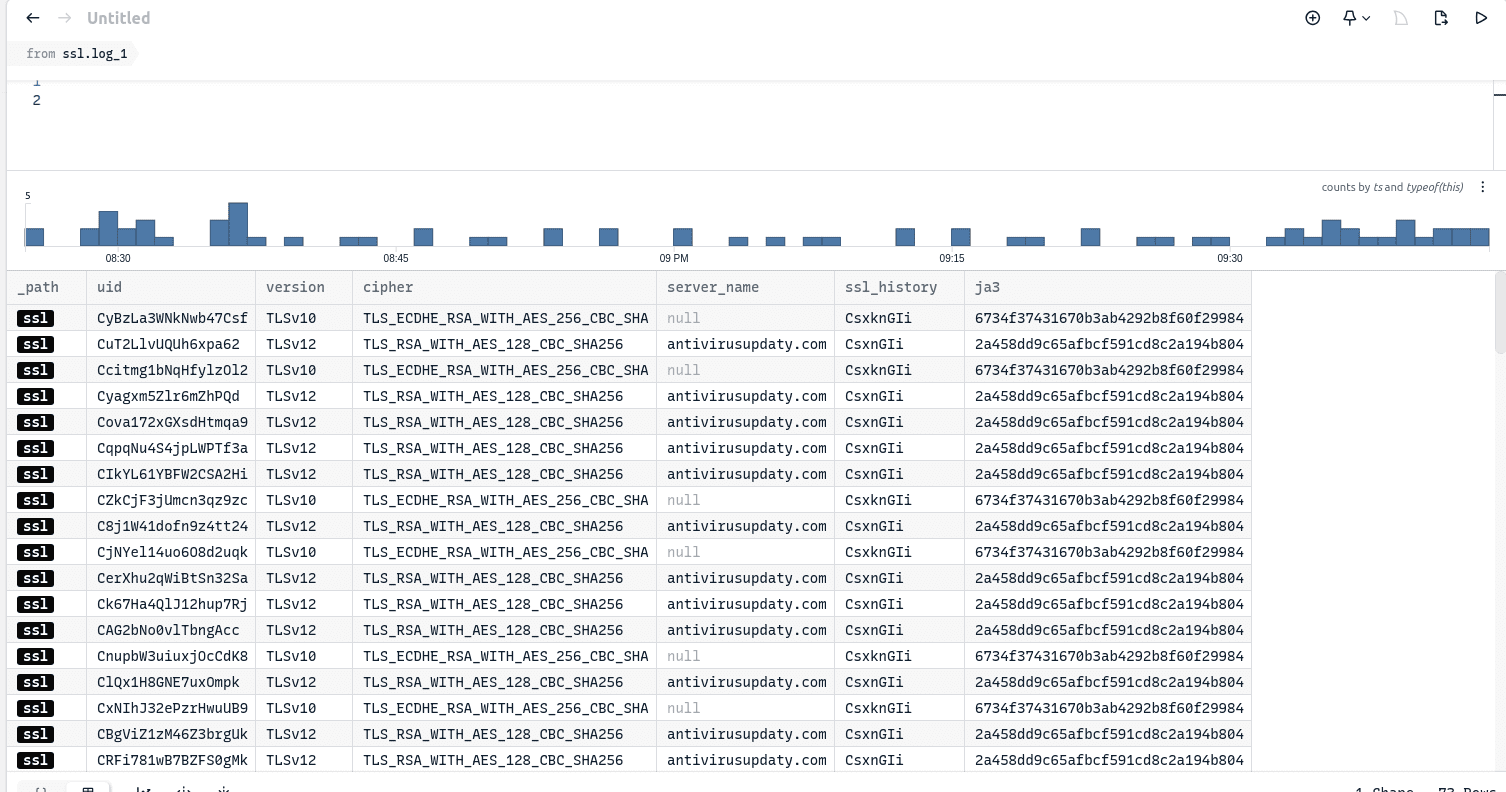
\includegraphics[width=1\linewidth]{images//ja3image/31.PNG}
    \caption{ssl.log in BRIM}
    \label{fig:enter-label}
\end{figure}

\begin{itemize}
    \item  The notice.log file is checked for Trickbot hash detection alerts, confirming the identification of malicious communications.\\\\
    JA3 = 6734f37431670b3ab4292b8f60f29984 ( Fingerprint of Trickbot )
\end{itemize}
\begin{figure}[H]
    \centering
    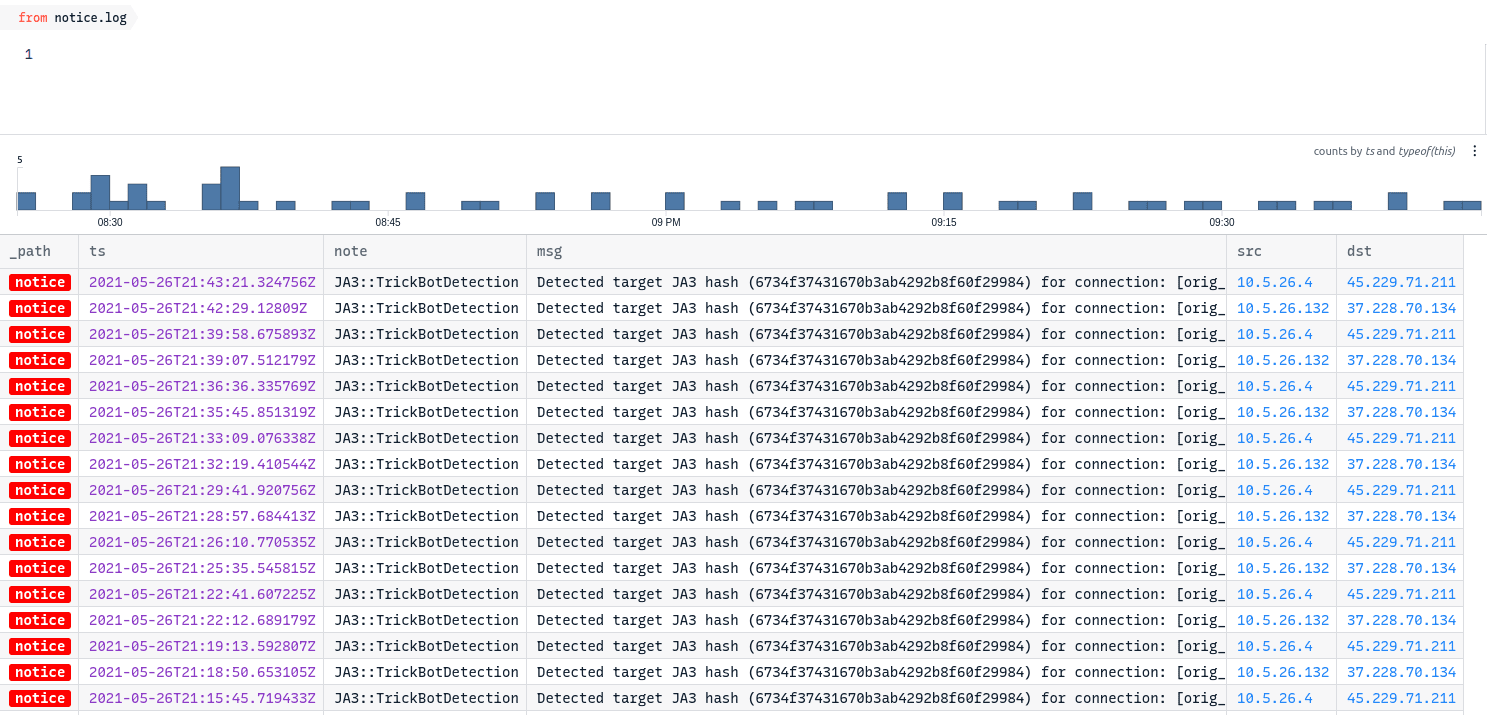
\includegraphics[width=1\linewidth]{images//ja3image/32.PNG}
    \caption{notice.log in BRIM}
    \label{fig:enter-label}
\end{figure}

\section{File Extraction and Hash Computation in Zeek}
\subsection{How It Works}
The process of file extraction in Zeek can be summarized as follows:
\begin{enumerate}
  \item \textbf{Event Detection:} Zeek scripts react to network events, such as the presence of a file in the network stream.
  \item \textbf{File Type Identification:} The script identifies the type of the file using its MIME type, enabling appropriate handling.
  \item \textbf{File Handling:} Based on the identified type, the script determines the handling procedure and naming convention for the file.
  \item \textbf{Analyzer Usage:} File analyzers, especially the extraction analyzer, are utilized to automatically save the file to the disk.
  \item \textbf{Extraction Configuration:} Specific parameters, such as the output filename, are defined for the extraction process.

\end{enumerate}

\subsection{File Extraction Script : }

\begin{lstlisting}[language=Python, caption= File EXtraction Script]
event file_sniff(f: fa_file, meta: fa_metadata)
{
    if (!meta?$mime_type) return;
    local filename: string;
    switch (meta$mime_type) {
        case "text/plain":
            print fmt("Detected Text file: %s", f$id);
            filename = fmt("extracted_text_%s.txt", f$id);
            break;
            
        case "text/html":
            print fmt("Detected HTML file: %s", f$id);
            filename = fmt("extracted_html_%s.html", f$id);
            break;
            
        case "image/png":
            print fmt("Detected PNG file: %s", f$id);
            filename = fmt("extracted_png_%s.png", f$id);
            break;

        default:
            return;
    }
    Files::add_analyzer(f, Files::ANALYZER_MD5);
    Files::add_analyzer(f, Files::ANALYZER_EXTRACT, [$extract_filename=filename]);
    
    print fmt("File will be extracted to: %s", filename);
}

event file_hash(f: fa_file, kind: string, hash: string)
{
    if (kind == "MD5")
    {
        print fmt("MD5 hash of file %s: %s", f$id, hash);
    }
}

event zeek_init()
{
    print "Zeek FILE Monitoring Script Initialized.";
}

\end{lstlisting}

\subsection{Script Explanation}
\begin{enumerate}
    \item \textbf{Event Detection} (Line 1) : Triggered by the \texttt{file\_sniff} event, the script processes each file detected in network traffic.
    \item \textbf{MIME Type Check} (Lines 3-19) The script exits the function early if a file does not have a MIME type associated with it.
    \item \textbf{File Classification} (Lines 3-19) : Files are classified based on their MIME type (text, HTML, PNG) and assigned unique filenames.
    \item \textbf{Analyzer Addition} (Lines 24-25) : The script adds MD5 and extraction analyzers for hashing and saving the files, respectively.
    \item \textbf{Extraction Notification} (Line 27) It logs the path where the file will be extracted to.
    \item \textbf{Hash Event} (Lines 30-36) : During the \texttt{file\_hash} event, the MD5 hash of the file is logged.
    \item \textbf{Initialization} (Lines 38-40) : The \texttt{zeek\_init} event signals that the script is ready for file monitoring.
\end{enumerate}

\subsection{Simulation}

We will commence by extracting files through a script that operates on both live network monitoring data and pre-captured pcap files.
\subsubsection{File Extraction from Live Network}
    \begin{itemize}
    \item The initial step involves locating the Zeek executable on the system.
    \end{itemize}
    \begin{figure}[H]
    \centering
    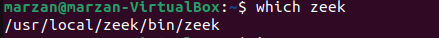
\includegraphics[width=1\linewidth]{images/which_zeek.png}
    \caption{zeek path}
    \label{fig:enter-label}
\end{figure}

     \begin{itemize}
     \item Subsequently, we will identify the active network interface on the machine to monitor the network traffic.
      \end{itemize}
    \begin{figure}[H]
    \centering
    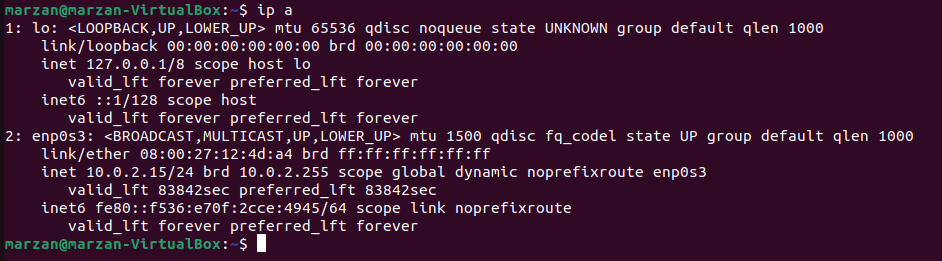
\includegraphics[width=1\linewidth]{images/ipa.png}
    \caption{active network interfaces}
    \label{fig:enter-label}
\end{figure}
\begin{itemize}

\item Following this, we initiate monitoring on the selected interface (enp0s3) using Zeek, which results in the extraction of 2 PDF files from the network traffic
 \end{itemize}
\begin{figure}[H]
    \centering
    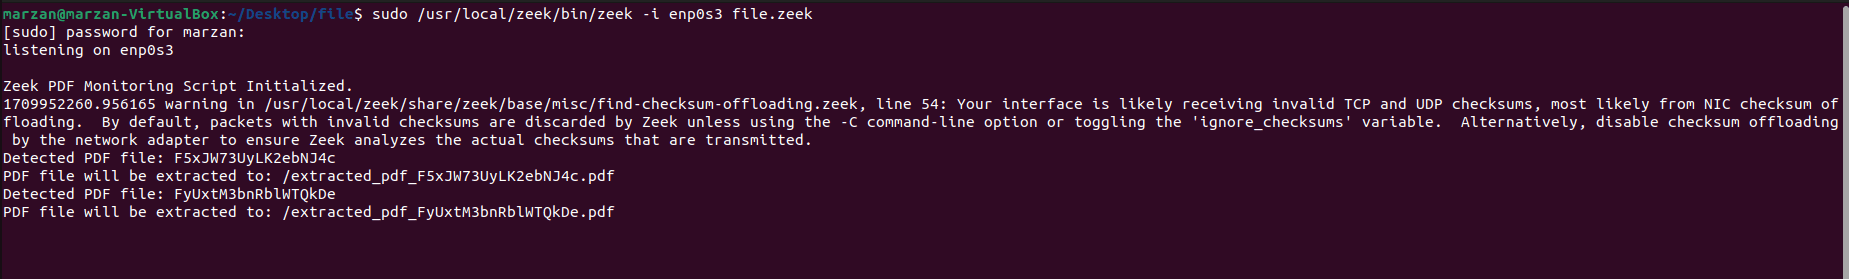
\includegraphics[width=1\linewidth]{images//extract_file/enpos3_file.png}
    \caption{PDF file extraction from live network monitoring}
    \label{fig:enter-label}
\end{figure}

\subsubsection{File Extraction from PCAP file}
\begin{itemize}
\item The same extraction process can be applied to pre-captured pcap files containing file transfer traffic\\\\
For this exercise, a pcap file is available at
PCAP file URL : \url{https://www.cloudshark.org/captures/a9472fbe700a}\\
The file can be downloaded by selecting "Export | Download".\\\\

By analyzing the pcap file with Zeek, we can extract files embedded within the network traffic.
The extracted files, which include a PNG file and a TXT file, are stored in the \textbf{/extract\_files} folder and are named according to their unique identifiers as logged by Zeek.
 \end{itemize}
\begin{figure}[H]
    \centering
    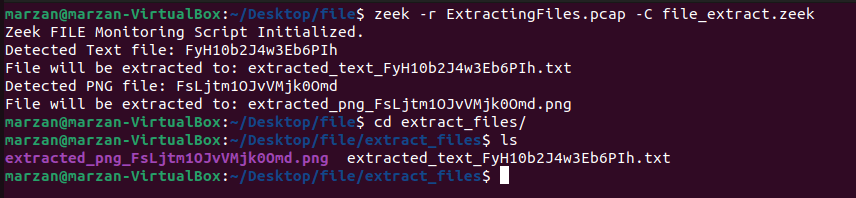
\includegraphics[width=1\linewidth]{images//extract_file/file_extract_1.png}
    \caption{PDF file extraction from pcap file}
    \label{fig:enter-label}
\end{figure}

\begin{itemize}
\item The \textbf{extract\_files} folder contains the two files that were extracted from the pcap file, showcasing Zeek's file extraction capabilities.
 \end{itemize}
\begin{figure}[H]
    \centering
    \includegraphics[width=0.5\linewidth]{images//extract_file/file_extract_2.png}
    \caption{Files inside extract\_files folder}
    \label{fig:enter-label}
\end{figure}

\begin{itemize}
\item A PNG file has been successfully extracted from the network traffic.

 \end{itemize}
\begin{figure}[H]
    \centering
    \includegraphics[width=0.5\linewidth]{images//extract_file/file_extract_3.png}
    \caption{PNG file}
    \label{fig:enter-label}
\end{figure}

\begin{itemize}
\item A TXT file has been successfully extracted from the network traffic.

 \end{itemize}
\begin{figure}[H]
    \centering
    \includegraphics[width=1\linewidth]{images//extract_file/file_extract_4.png}
    \caption{TXT file}
    \label{fig:enter-label}
\end{figure}

\begin{itemize}
\item Additionally, the files.log file, which can be viewed in BRIM, provides an MD5 hash value for each extracted file, facilitating further analysis and verification of the files' integrity.

 \end{itemize}
\begin{figure}[H]
    \centering
    \includegraphics[width=1\linewidth]{images//extract_file/file_extract_5.png}
    \caption{files.log in BRIM}
    \label{fig:enter-label}
\end{figure}



\section{Malware Hash Detection in Zeek}
\subsection{How It Works}
The Zeek script integrates with Team Cymru's Malware Hash Registry to enhance network security monitoring by identifying files with hash values known to be associated with malware. The process is outlined as follows:

\begin{itemize}

    \item \textbf{Initialization :} The script initializes by loading essential frameworks for file handling and notice management, setting the groundwork for its operations.
    \item \textbf{Notice Extension :} It extends Zeek's notice mechanism to include a new type specifically for malware hash matches, facilitating targeted alerts.
    \item \textbf{File Filtering :} File downloads are filtered by MIME type, focusing the analysis on file formats commonly associated with malware dissemination.
    \item \textbf{Malware Hash Lookup :} For each relevant file, the script performs a DNS TXT lookup against the Malware Hash Registry using the file's SHA-1 hash as the query, efficiently leveraging external threat intelligence.
    \item \textbf{Lookup Evaluation :} The lookup response, containing the detection rate and first detection date, is evaluated against a predefined threshold to determine the file's potential threat level.
    \item \textbf{Notice Generation :} If the detection criteria are met, a notice is generated, including the malware detection rate, the URL for further information, and the file's last seen date, thereby informing the network administrator of potential security threats.
    \item \textbf{Network Defense Enhancement :} This integration allows for an automated, real-time response to the transmission of potentially malicious files, enhancing the network's defensive posture against malware.
\end{itemize}


\subsection{Detect-MHR Script:}
\begin{lstlisting}[language=Python, caption=detect-MHR.zeek]
##! Detect file downloads that have hash values matching files in Team
##! Cymru's Malware Hash Registry (https://www.team-cymru.com/mhr.html).

@load base/frameworks/files
@load base/frameworks/notice
@load frameworks/files/hash-all-files

module TeamCymruMalwareHashRegistry;

export {
	redef enum Notice::Type += {
		Match
	};

	## File types to attempt matching against the Malware Hash Registry.
	option match_file_types = /application\/x-dosexec/ |
	                         /application\/vnd\.ms-cab-compressed/ |
	                         /application\/pdf/ |
	                         /application\/x-shockwave-flash/ |
	                         /application\/x-java-applet/ |
	                         /application\/jar/ |
	                         /video\/mp4/;


	option match_sub_url = "https://www.virustotal.com/gui/search/%s";
	option notice_threshold = 10;
}


function do_mhr_lookup(hash: string, fi: Notice::FileInfo)
	{
	local hash_domain = fmt("%s.malware.hash.cymru.com", hash);
	when [hash, fi, hash_domain] ( local MHR_result = lookup_hostname_txt(hash_domain) )
		{
		local MHR_answer = split_string1(MHR_result, / /);

		if ( |MHR_answer| == 2 )
			{
			local mhr_detect_rate = to_count(MHR_answer[1]);
			if ( mhr_detect_rate >= notice_threshold )
				{
				local mhr_first_detected = double_to_time(to_double(MHR_answer[0]));

				local readable_first_detected = strftime("%Y-%m-%d %H:%M:%S", mhr_first_detected);

				local message = fmt("Malware Hash Registry Detection rate: %d%%  Last seen: %s", mhr_detect_rate, readable_first_detected);

				local virustotal_url = fmt(match_sub_url, hash);

				local n: Notice::Info = Notice::Info($note=Match, $msg=message, $sub=virustotal_url);
				Notice::populate_file_info2(fi, n);
				NOTICE(n);
				}
			}
		}
	}

event file_hash(f: fa_file, kind: string, hash: string)
	{
	if ( kind == "sha1" && f?$info && f$info?$mime_type &&
	     match_file_types in f$info$mime_type )
		do_mhr_lookup(hash, Notice::create_file_info(f));
	}

 \end{lstlisting}

 \subsection{Detect-MHR Script Explanation :}
 \begin{enumerate}
    \item \textbf{Module and Dependencies} (Lines 4-8) : The script introduces the `TeamCymruMalwareHashRegistry` module and includes necessary Zeek frameworks for file operations and notice generation.
    \item \textbf{Notice Type Extension} (Lines 11-12) : Extends `Notice::Type` with `Match` to signify malware hash matches.
    \item \textbf{File Type Filtering} (Lines 16-22) : Defines `match\_file\_types` to specify MIME types of interest, including executables, archives, PDFs, Flash, Java applets, and MP4 videos.
    \item \textbf{Malware Information URL} (Line 25) : The `match\_sub\_url` option formats a URL to VirusTotal, substituting `%s` with the file's SHA-1 hash for further investigation.
    \item \textbf{Detection Threshold} (Line 26) : Sets a `notice\_threshold` to determine the minimum detection rate by antivirus engines for generating a notice.
    \item \textbf{Malware Hash Lookup} (Lines 30-48) : Implements `do\_mhr\_lookup` to query the hash in Team Cymru's Malware Hash Registry via DNS TXT lookup.
    \item \textbf{Handling Lookup Results} (Lines 50-52) : Processes lookup results, generating a notice if the detection rate exceeds the set threshold, including the rate, last seen date, and a VirusTotal link.
    \item \textbf{File Hash Event} (Lines 58-62) : The `file\_hash` event initiates the malware hash lookup for SHA-1 hashes of files matching the specified MIME types.
\end{enumerate}

\subsection{Simulation : }
Here is the link to VirusTotal: \href{https://www.virustotal.com/gui/search/a38b59afb1f03b2c2cfc14ae5a953d8e5fd6b56d}{VirusTotal}\\
Here is the link to PCAP file:
\href{https://www.malware-traffic-analysis.net/tutorials/index.html}{malware-traffic-analysis}\\\\
\begin{itemize}
    \item To begin the analysis, the malicious pcap file is processed using the detect-MHR.zeek script, specifically designed for malware hash detection.
\end{itemize}

\begin{figure}[h!]
    \centering
    \includegraphics[width=1\linewidth]{images//file_malware/file_malware_1.png}
    \caption{Running PCAP with Script}
    \label{fig:enter-label}
\end{figure}

\begin{itemize}
    \item The notice.log entries highlight malware detections with the following critical information: the detection rate, the last seen date, and a link to VirusTotal for further investigation. For instance, one entry shows a 3\% detection rate for malware last seen on 2021-06-22, with a corresponding VirusTotal search link for the hash bdfb8b29614001dfe9922524c910ee4badb0e6fc. Another entry indicates a 32\% detection rate for malware last seen on 2021-06-04, linked to the hash 9b4025714911d509a67423ed8beffbc49e54845d on VirusTotal. These details facilitate a deeper analysis of the detected threats.
\end{itemize}
\begin{figure}[H]
    \centering
    \includegraphics[width=1\linewidth]{images//file_malware/file_malware_2.png}
    \caption{notice.log}
    \label{fig:enter-label}
\end{figure}

\begin{itemize}
    \item These detection logs can be viewed in a tabular format within the BRIM application, providing a user-friendly interface for detailed analysis.
\end{itemize}
\begin{figure}[H]
    \centering
    \includegraphics[width=1\linewidth]{images//UDP_reflection/file_malware_6.png}
    \caption{notice.log in BRIM}
    \label{fig:enter-label}
\end{figure}

\begin{figure}[H]
    \centering
    \includegraphics[width=1\linewidth]{images//UDP_reflection/file_malware_7.png}
    \caption{notice.log in BRIM}
    \label{fig:enter-label}
\end{figure}

\begin{itemize}
    \item Within BRIM, each entry's detailed information is accessible, including path, timestamp, unique identifiers, file information, MIME type, descriptions, protocols, notices, messages, source and destination details, and more. This detailed view aids in a comprehensive analysis of each detected event.
\end{itemize}
\begin{figure}[H]
    \centering
    \includegraphics[width=0.7\linewidth]{images//file_malware/file_malware_3.png}
    \caption{Entries of notice.log in BRIM}
    \label{fig:enter-label}
\end{figure}

\begin{itemize}
    \item Following the links in the notice.log to VirusTotal provides a detailed security report for each file hash, including the community score, detection rates by various security vendors, and additional malware characteristics. This external validation offers insights into the potential threats and the behavior of the detected files.
\end{itemize}
\begin{figure}[H]
    \centering
    \includegraphics[width=1\linewidth]{images//file_malware/file_malware_4.png}
    \caption{VirusTotal Page Showing Malicious Percentage}
    \label{fig:enter-label}
\end{figure}

\begin{itemize}
    \item The VirusTotal reports also reveal basic file properties such as MD5, SHA-1, and SHA-256 hashes, providing an authoritative fingerprint of the files for cross-reference and further investigation into their origins, distribution, and impact.
\end{itemize}
\begin{figure}[H]
    \centering
    \includegraphics[width=1\linewidth]{images//file_malware/file_malware_5.png}
    \caption{VirusTotal Page Showing File Info}
    \label{fig:enter-label}
\end{figure}

\section{Codebase Structure}
Zeek (formerly Bro) is an open-source framework for network analysis, security monitoring, and forensics. Developed with contributions from many developers and led by key contributor Vern Paxson, a UC Berkeley professor, it has become a vital tool in the computer security community.
\subsection{Language :}
Zeek is primarily written in C++ and uses scripting languages for its analysis scripts. The transition to C++ has allowed Zeek to leverage the performance and efficiency of compiled languages, making it highly suitable for high-speed network environments.

\subsection{Repository}
The source code for Zeek is hosted on GitHub, making it accessible for community contributions, issue tracking, and feature requests.
\begin{itemize}
\item Access URL: \url{https://github.com/zeek/zeek}
\item Repository Owner: Zeek
\end{itemize}

\subsection{Key Components}
\begin{enumerate}
    \item \textbf{Packet Capture and Analysis Engine}: : Optimized with C++ for high-throughput network traffic processing, featuring selective data filtering and modular protocol analysis capabilities.
    \item \textbf{Event Engine}: Built on a C++ publish-subscribe model, it efficiently generates and dispatches network events, separating event creation from processing for flexible script execution
    \item \textbf{Scripting Language Interpreter}: Integral to Zeek, it executes analysis scripts, offering direct access to network events and data, and supports dynamic script management.
    \item \textbf{Logging Framework}: Versatile logging system supporting multiple formats like JSON, CSV, and script-driven customization for tailored data recording
    \item \textbf{Plugin Architecture}: Allows dynamic plugin integration without Zeek restarts, offering APIs for seamless extension of core functionalities
    \item \textbf{Analysis Scripts and Signature Database}: : Runtime-loaded scripts in Zeek's language define detection logic and extend analysis, with a signature database identifying network threats.
  
    
\end{enumerate}
\subsection{Directories and Major Files :}
\subsubsection{/src - Core C++ Code}
\begin{itemize}
    \item \textbf{analyzer/}: Protocol analyzers dissect network protocols to generate events.
    \begin{itemize}
        \item \emph{ProtocolAnalyzer.cc / .h}: Base classes for protocol analyzers.
        \item Protocol-specific subdirectories (e.g., \emph{http/}, \emph{dns/}) contain implementations for each analyzer.
    \end{itemize}

    \item \textbf{file\_analysis/}: Framework for file extraction and analysis.
    \begin{itemize}
        \item \emph{File.cc / .h}: Core classes for file analysis.
        \item \emph{Analyzer.cc / .h}: Base and implementation classes for file analyzers.
    \end{itemize}

    \item \textbf{iosource/}: Input sources management, including packet capture.
    \begin{itemize}
        \item \emph{PktSrc.cc / .h}: Abstract base for packet sources.
        \item \emph{PcapSrc.cc / .h}: pcap-based packet source implementation.
    \end{itemize}

    \item \textbf{logging/}: Zeek's structured logging framework.
    \begin{itemize}
        \item \emph{WriterFrontend.cc / .h}: Interfaces for log writers.
        \item \emph{writers/}: Implementations for various log output formats.
    \end{itemize}

    \item \emph{main.cc}: Main entry point, initializing the environment and starting the processing loop.
    
    \item \emph{net\_util.cc / .h}: Network utility functions for address manipulation.

    \item \textbf{policy/}: Script-level policy handlers for security policies and detections.

    \item \emph{Reporter.cc / .h}: Reporting of warnings, errors, and runtime messages.

    \item \textbf{script\_opt/}: Script execution optimizations for performance.

    \item \textbf{threading/}: Manages threading and concurrency for parallelized operations.
\end{itemize}

\subsubsection{/scripts - Zeek Script Library}
\begin{itemize}
    \item \textbf{base/}: Default behaviors, protocol parsing, and logging scripts.
    \begin{itemize}
        \item \emph{protocols/}: Scripts for network protocol handling.
        \item \emph{frameworks/}: Core frameworks like logging, notices, and file analysis.
    \end{itemize}
    \item \textbf{policy/}: Optional scripts for feature extensions or behavior modifications.
\end{itemize}

\subsubsection{/aux - Auxiliary Tools and Scripts}
Tools and scripts supporting Zeek's core functionality, aiding in tasks like plugin development, testing, or integration.

\subsubsection{/testing - Testing Framework and Suites}
\begin{itemize}
    \item \emph{btest/}: BTest testing framework scripts.
    \item \emph{Traces/}: Network trace files for testing protocol analyzers and script behaviors.
    \item \emph{Scripts/}: Defines test cases and expected outcomes.
\end{itemize}

\subsubsection{/doc - Documentation}
Zeek's documentation, including user guides, developer documentation, and API references, primarily in reStructuredText format.

\subsubsection{/cmake - Build System Configurations}
CMake configurations and scripts for compiler options, dependencies, and build targets.

\subsubsection{/zeekctl - Command-Line Control Interface}
(For older versions) Contains `zeekctl` scripts and configurations. In newer versions, `zeekctl` is a separate project.

\subsubsection{Plugin Support}
Framework for extending Zeek's capabilities via plugins, typically developed in separate repositories or directories.



\section{References}
Below are the key resources for Zeek, a powerful network analysis framework:\\
\begin{itemize}
   

 \item  Zeek Official Website: \href{https://zeek.org}{https://zeek.org}\\

 \item  Zeek Documentation: Detailed information about Zeek can be found on their documentation site at \href{https://docs.zeek.org/en/master/}{https://docs.zeek.org/en/master/}\\

 \item  Zeek GitHub Repository: For source code and development resources, visit Zeek's GitHub page at \href{https://github.com/zeek/zeek}{https://github.com/zeek/zeek}\\


\end{itemize}
\end{document}
